\ifx\wholebook\relax \else

\documentclass[b5paper]{ctexart}
\usepackage[nomarginpar
  %, margin=.5in
]{geometry}

\addtolength{\oddsidemargin}{-0.05in}
\addtolength{\evensidemargin}{-0.05in}
\addtolength{\textwidth}{0.1in}

\usepackage[cn]{../prelude}

\setcounter{page}{1}

\begin{document}

\title{无理数}

\author{刘新宇
\thanks{{\bfseries 刘新宇} \newline
  Email: liuxinyu99@hotmail.com \newline}
  }

\maketitle
\fi

\markboth{无理数}{数的旅程}

\ifx\wholebook\relax
\chapter{无理数}
\fi

\epigraph{数学是上帝用来书写宇宙的文字}{伽利略}

公元前240年的夏至中午,这一天是一年中日照最长的一日,大约是现代历法的6月21日附近。埃及亚历山大港图书馆馆长埃拉托斯特尼(公元前276年~194年)正和一位来自赛印城的商人交谈。赛印(Syene)位于今天埃及南部的阿斯旺,是北回归线上的一个城市。“我的老家是世上最干最热的地方。”商人说道:“我们打了很深的井汲水,每年的这个时候,阳光能射到井底呢。”听到这句话时埃拉托斯特尼注意到了到广场上纪念碑的影子。为什么会这样呢?除非大地不是平坦的,而是球形。他询问哪个商人:“从赛印城到亚历山大有多远的路程?”“有5000斯塔蒂亚。”斯塔蒂亚(Stadia)是古希腊的长度单位,约和158米。埃拉托色特尼测量了立在地上的杆子和影子的长度,发现杆子的长度大约是影子长度的8倍。他于是按照\cref{fig:eratosthenes-earth}进行了计算。

\begin{figure}[htbp]
 \centering
 \subcaptionbox{太阳在夏至直射北回归线上的赛印城\label{fig:eratosthenes-earth}}{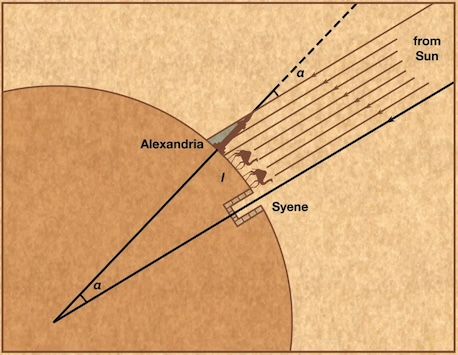
\includegraphics[scale=0.35]{img/eratosthenes-earth}}
 \subcaptionbox{太阳照射亚历山大的角度为$\alpha$\label{fig:atan8}}{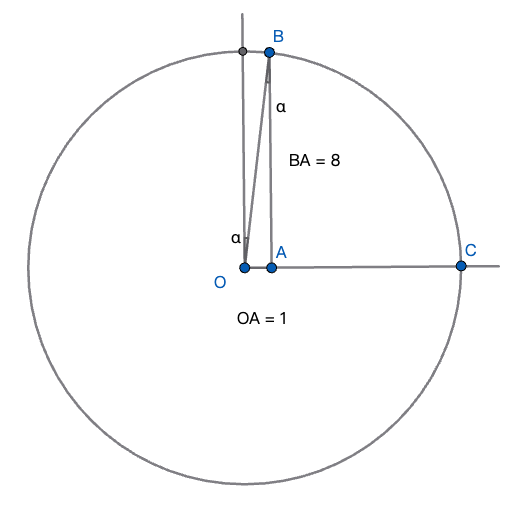
\includegraphics[scale=0.32]{img/atan8}}
 \caption{埃拉托斯特尼测量地球}
\end{figure}

夏至正午时刻,太阳直射北回归线,因此阳光可以射入赛印城的井底。埃拉托色特尼可以通过\cref{fig:atan8}找出阳光照射亚历山大港的角度。
%% 这相当于今天高中数学中的反正切$\arctan(\frac{1}{8})$。
但当时古巴比伦的角度单位还没有传入古希腊,按照埃拉托斯特尼的说法,这个角度是圆的50分之一,合$7.2\degree$。太阳光是平行光。如果大地是球形的,那么赛印城和亚历山大到球心的张角,是太阳入射角的同位角(\cref{fig:eratosthenes-earth}中标有$\alpha$的两个角),也是圆的50分之一。所以赛印城到亚历山大之间的距离就是地球周长的50分之一。这样算来,地球的周长就是$50 \times 5000 = 250000$斯塔提雅,约合$250 \times 158 = 39500 \approx 4$万千米。而今天人们通过人造卫星测得地球赤道长度为40075千米。埃拉托色特尼的著作没有流传到今天,我们从古希腊数学家帕普斯等人的记述中了解到他的具体测量方法。埃拉托色特尼约在公元前235年起任亚历山大图书馆馆长,他对地球的测量发生在这一时期\cite{Walkup2005}。赛印城到亚历山大的距离是一个关键,5000斯塔蒂亚无疑是一个大致数字。埃拉托斯特尼可能通过多种途径核证该距离,包括询问往来的商人以及测量地图。赛印城和亚历山大港都是尼罗河沿岸城市,尼罗河有规律的每年泛滥,埃及人因此每年在泛滥后重新丈量尼罗河沿线的土地并更新地图。此外,古希腊的斯塔蒂亚到底有多长学者们也有不同的观点。无论如何,埃拉托色特尼在2000年前的伟大推理和计算无疑是惊人的。

\begin{figure}[htbp]
 \centering
 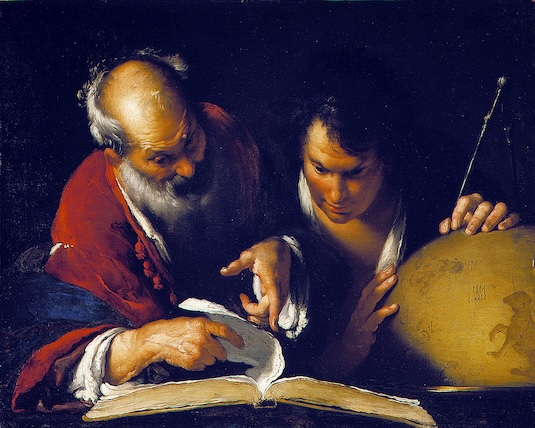
\includegraphics[scale=0.35]{img/eratosthenes}
 % https://commons.wikimedia.org/wiki/File:Eratosthenes_Teaching_in_Alexandria_(Bernardo_Strozzi,_Montreal).jpg
 \caption{贝尔纳多·斯特罗齐于1635年创作的油画:在亚历山大教学的埃拉托色特尼}
 \label{fig:eratosthenes}
\end{figure}

马其顿国王亚历山大大帝征服埃及后,兴建了以他命名的城市亚历山大港,成为了希腊化时代的文化和学术中心。埃拉托色特尼测量地球的壮举通常被认为是体现古希腊几何学力量的典范。古希腊并没有位值制计数系统(见第1章),但却发展出了严密的推理和几何学传统。正是在把数和几何学结合后,古希腊人\underdot{发现}了无理数,使得数的大家庭又得到了一次扩充。

\section{万物皆数}
音乐与数似乎毫无关联,但毕达哥拉斯却发现了它们背后竟有奇妙的规律。他从中得到启发并大胆推测“万物皆数”(All is number),认为世间万物都可以用数或数的比例来理解。毕达哥拉斯可以说是用数探索世间万物的第一人。他出生于希腊的萨摩斯(Samos)岛,年轻时他曾去米利都(Miletus)向古希腊哲学的奠基人泰勒斯(Thales)学习。在泰勒斯的建议下,毕达哥拉斯于公元535年前往埃及学习数学。公元前525年,波斯帝国征服了埃及,他被俘并随军向东到达了巴比伦。毕达哥拉斯得以向巴比伦人学习数学和天文知识。或许后来他还到达了更远的印度。不论到了哪里,毕达哥拉斯都不断向有学问的人请教,丰富自己的见解。重要的是,他不仅刻苦学习,而且更善于思考。在经过兼收并蓄、汲取各家之长后,毕达哥拉斯形成并完善了自己的思想\cite{HanXueTao16}。

经历了漫长的在外游历后,年近半百的毕达哥拉斯返回了故乡萨默斯并开始讲学。公元前520年左右,也许为了摆脱当地的暴政,毕达哥拉斯移居到了意大利南部的克罗顿(Croton)发展。在那里他赢得了人们的信任与景仰并形成了自己的学派。毕达哥拉斯的弟子中还有女性,学派把主要精力都用来研究天文、几何、数论、音乐这四门学科。它们被称为四术(quadrivium),影响了欧洲教育两千多年\cite{StepanovRose15}。四术体现了毕达哥拉斯万物皆数的哲学思想:星体的运动与几何对应,而几何又以数为基础,数字还可以衍生出音乐(见第3章)。关于毕达哥拉斯去世有多种说法。他领导的学派具有很高的声誉和政治影响,引起了敌对派的忌恨。约公元前497年,学派在克罗顿的活动场所遭到破坏。有人认为毕达哥拉斯被暴徒杀害,也有人说他逃到梅塔蓬图姆(Metapontum)并度过余生\cite{MKlein1972}。

\index{形数(figurate number)}
毕达哥拉斯学派研究数字,认为数与数、数与自然之间存在着神秘关系。这开启了数学的重要分支——数论。学派对正整数进行了分类,定义了奇数、偶数、素数、合数等。他们通过在地上摆小石子来研究数字,英文的计算calculus一词就是从希腊文“石子”衍生出的\cite{HanXueTao16}。当把石子按照某种几何图形摆放时,就得到了形数(figurate number)。

\begin{figure}[htbp]
%\begin{wrapfigure}{R}{0.4\textwidth}
\centering
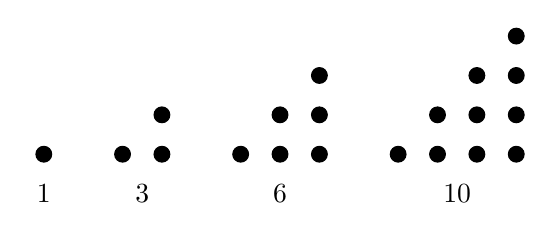
\begin{tikzpicture}[scale=0.5]
\filldraw (0, 0) circle (0.2);
\draw (0, -1) node{1};
\filldraw (2, 0) circle (0.2)
          (3, 0) circle (0.2)   (3, 1) circle (0.2);
\draw (2.5, -1) node{3};
\filldraw (5, 0) circle (0.2)
          (6, 0) circle (0.2)   (6, 1) circle (0.2)
          (7, 0) circle (0.2)   (7, 1) circle (0.2)   (7, 2) circle (0.2);
\draw (6, -1) node{6};
\filldraw (9, 0) circle (0.2)
          (10, 0) circle (0.2)    (10, 1) circle (0.2)
          (11, 0) circle (0.2)    (11, 1) circle (0.2)    (11, 2) circle (0.2)
          (12, 0) circle (0.2)    (12, 1) circle (0.2)    (12, 2) circle (0.2)    (12, 3) circle (0.2);
\draw (10.5, -1) node{10};
\end{tikzpicture}
\caption{三角形数(triangular number)}
\label{fig:triangular-num}
%\end{wrapfigure}
\end{figure}

\begin{figure}[htbp]
%\begin{wrapfigure}{R}{0.4\textwidth}
\centering
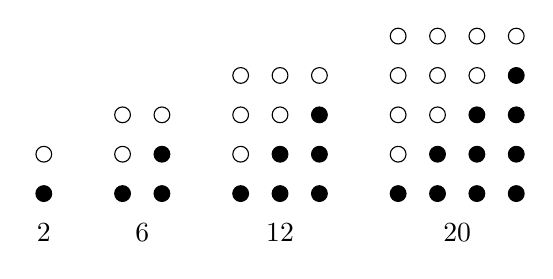
\begin{tikzpicture}[scale=0.5]
\draw (0, 1) circle (0.2);
\filldraw (0, 0) circle (0.2);
\draw (0, -1) node{2};

\draw (2, 1) circle (0.2)   (2, 2) circle (0.2)
      (3, 2) circle (0.2);
\filldraw (2, 0) circle (0.2)
          (3, 0) circle (0.2)   (3, 1) circle (0.2);
\draw (2.5, -1) node{6};

\draw (5, 1) circle (0.2)   (5, 2) circle (0.2)   (5, 3) circle (0.2)
      (6, 2) circle (0.2)   (6, 3) circle (0.2)
      (7, 3) circle (0.2);
\filldraw (5, 0) circle (0.2)
          (6, 0) circle (0.2)   (6, 1) circle (0.2)
          (7, 0) circle (0.2)   (7, 1) circle (0.2)   (7, 2) circle (0.2);
\draw (6, -1) node{12};

\draw (9, 1) circle (0.2)   (9, 2) circle (0.2)   (9, 3) circle (0.2)   (9, 4) circle (0.2)
      (10, 2) circle (0.2)   (10, 3) circle (0.2)   (10, 4) circle (0.2)
      (11, 3) circle (0.2)   (11, 4) circle (0.2)
      (12, 4) circle (0.2);
\filldraw (9, 0) circle (0.2)
          (10, 0) circle (0.2)    (10, 1) circle (0.2)
          (11, 0) circle (0.2)    (11, 1) circle (0.2)    (11, 2) circle (0.2)
          (12, 0) circle (0.2)    (12, 1) circle (0.2)    (12, 2) circle (0.2)    (12, 3) circle (0.2);
\draw (10.5, -1) node{20};
\end{tikzpicture}
\caption{长方形数(oblong number)}
\label{fig:oblong-num}
%\end{wrapfigure}
\end{figure}

\cref{fig:triangular-num}和\cref{fig:oblong-num}分别是三角形数和长方形数。容易看出,每个长方形数都对应三角形数的二倍,而三角形数又是前$n$个正整数之和,这样就得到了正整数累加的求和公式:

\[
1 + 2 + 3 + ... + n = \frac{1}{2}n(n+1)
\]

毕达哥拉斯学派还观察到,所有的奇数可以表示成折尺形(或称为“磬折形”)\footnote{gnomon这个字在巴比伦人的原意可能是指日晷上的直杆,用它的阴影来指示时刻。在毕达哥拉斯时代,gnomon指木匠用的方尺。它还表示从正方形的一角切掉一个小正方形后剩余的图形。以后欧几里得又把正方形扩展到平行四边形\citepage[26页]{MKlein1972}。},如\cref{fig:gnomon-num},而前$n$个折尺形可以拼成一个正方形,如\cref{fig:square-num}。这样他们就发现了前$n$个正奇数的求和公式:

\[
1 + 3 + 5 + ... + (2n - 1) = n^2
\]

\begin{figure}[htbp]
%\begin{wrapfigure}{R}{0.4\textwidth}
\centering
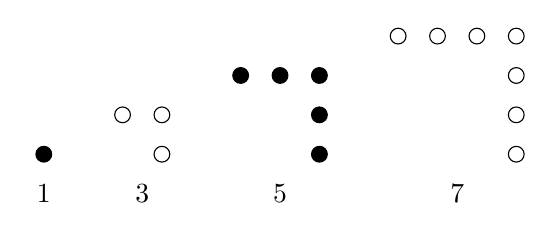
\begin{tikzpicture}[scale=0.5]
\filldraw (0, 0) circle (0.2);
\draw (0, -1) node{1};

\draw (2, 1) circle (0.2)
      (3, 0) circle (0.2)   (3, 1) circle (0.2);
\draw (2.5, -1) node{3};

\filldraw (5, 2) circle (0.2)   (6, 2) circle (0.2)   (7, 2) circle (0.2)
          (7, 0) circle (0.2)   (7, 1) circle (0.2);
\draw (6, -1) node{5};

\draw (9, 3) circle (0.2)   (10, 3) circle (0.2)   (11, 3) circle (0.2)   (12, 3) circle (0.2)
      (12, 0) circle (0.2)    (12, 1) circle (0.2)    (12, 2) circle (0.2);
\draw (10.5, -1) node{7};
\end{tikzpicture}
\caption{折尺形数(gnomon number)}
\label{fig:gnomon-num}
%\end{wrapfigure}
\end{figure}

\begin{figure}[htbp]
%\begin{wrapfigure}{R}{0.4\textwidth}
\centering
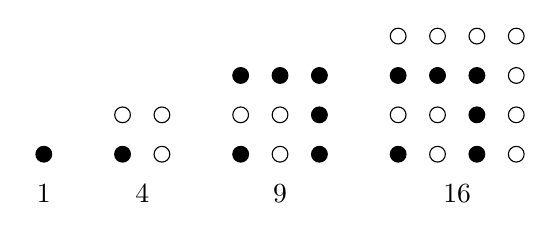
\begin{tikzpicture}[scale=0.5]
\filldraw (0, 0) circle (0.2);
\draw (0, -1) node{1};

\filldraw (2, 0) circle (0.2);
\draw (2, 1) circle (0.2)
      (3, 0) circle (0.2)   (3, 1) circle (0.2);
\draw (2.5, -1) node{4};

\filldraw (5, 0) circle (0.2);
\draw (5, 1) circle (0.2)
      (6, 0) circle (0.2)   (6, 1) circle (0.2);
\filldraw (5, 2) circle (0.2)   (6, 2) circle (0.2)   (7, 2) circle (0.2)
          (7, 0) circle (0.2)   (7, 1) circle (0.2);
\draw (6, -1) node{9};

\filldraw (9, 0) circle (0.2);
\draw (9, 1) circle (0.2)
      (10, 0) circle (0.2)   (10, 1) circle (0.2);
\filldraw (9, 2) circle (0.2)   (10, 2) circle (0.2)   (11, 2) circle (0.2)
          (11, 0) circle (0.2)   (11, 1) circle (0.2);
\draw (9, 3) circle (0.2)   (10, 3) circle (0.2)   (11, 3) circle (0.2)   (12, 3) circle (0.2)
      (12, 0) circle (0.2)    (12, 1) circle (0.2)    (12, 2) circle (0.2);
\draw (10.5, -1) node{16};
\end{tikzpicture}
\caption{正方形数(square number)与折尺形数的关系}
\label{fig:square-num}
%\end{wrapfigure}
\end{figure}

就这样,毕达哥拉斯学派把几何形状也建立在了数的基础上。他们热衷与用数去解释更多的现象,并相信宇宙的本质就在于“数的和谐”,由此出发,毕达哥拉斯学派试图发展一套以数字为基础的理论,使得几何学可以建立在该理论之上。

\section{勾股定理}

\begin{figure}[htbp]
 \centering
 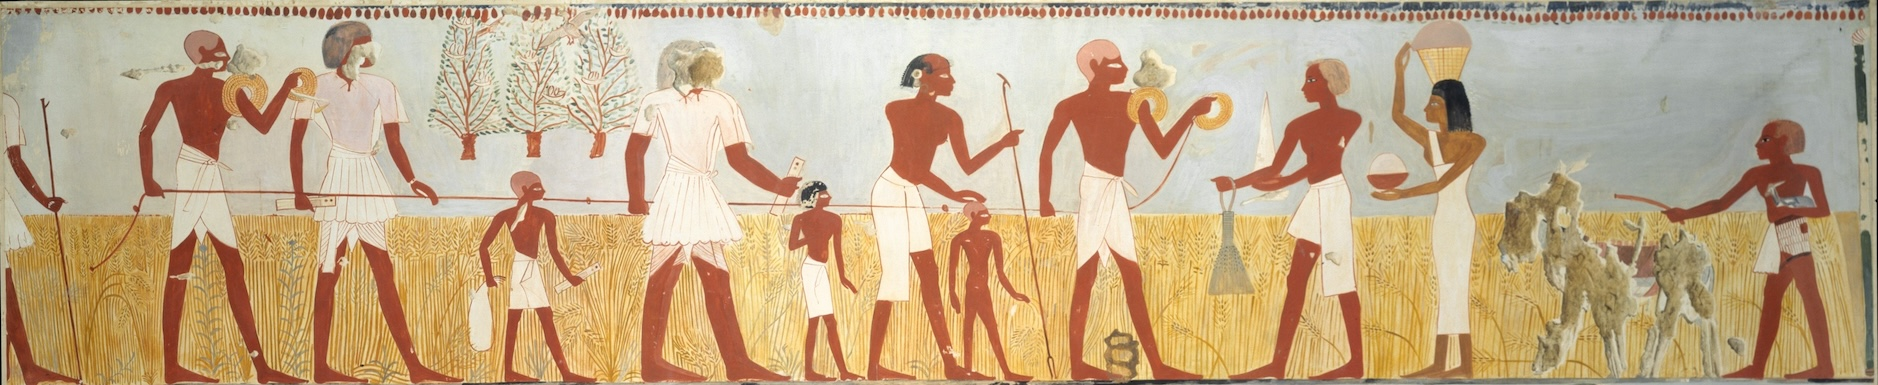
\includegraphics[scale=0.35]{img/harvest-scene}
 \caption{拉绳测量,来自梅纳陵墓壁画《收割场景》上半部分。梅纳是古埃及第十八王朝(公元前1400~1352年)的祭司和土地丈量官。现收藏于美国大都会艺术博物馆。}
 %% https://www.metmuseum.org/art/collection/search/548574
 \label{fig:rope-meter}
\end{figure}

毕达哥拉斯学派最著名的发现当属勾股定理,在西方叫做“毕达哥拉斯定理”。据说毕达哥拉斯对他发现的这个定理及其证明极为高兴,为此献祭了一百头公牛庆贺。但脍炙人口的传说故事往往不真实。毕达哥拉斯学派对团体成员有着极为严格的戒律,任何人的研究发现都归学派所有并必须保密。我们所知的以“毕达哥拉斯”命名的成果大都来自学派内的佚名作者。勾股定理并非孤立成果,各个文明都各自独立发现了它。如第3章中的\cref{fig:babylonian-yale}所示,这块古巴比伦泥板的时间大约是公元前1900年~1600年,此外人们还发现了刻有勾股数表的泥板。古埃及的测量员绳子作为软尺(称为拉绳人,见\cref{fig:rope-meter})。相传他们在绳上打结,把全长分成长度为3比4比5的三段,然后用来形成直角三角形。但这个说法没有文献证实\citepage[16页]{MKlein1972}。古印度数学家包德哈亚那(Baudhayana,生活在公元前800年到公元前400年间)的著作《绳法经》(Śulba Sutra)也提到了这个定理。在古代中国,成书于公元前一世纪的《周髀算经》中载有西周时代(约公元前11世纪)周公和商高的一段对话,其中提到“勾三、股四、弦五”\footnote{商高说:“……故折矩,勾广三,股修四,经隅五。”},故在中国称之为“勾股定理”。《九章算术》的注解中载有三国时代的赵爽和魏晋时刘徽给出的勾股定理证明\footnote{对赵爽和刘徽给出的究竟是严格意义的证明还是某种程度的解释历来有不同观点。}。

\begin{figure}[htbp]
 \centering
 \subcaptionbox{中国数学会会徽\label{fig:cms-logo}}{
\includegraphics[scale=0.5]{img/cms}} \quad
 \subcaptionbox{赵爽弦图\label{fig:zhaoshuang}}{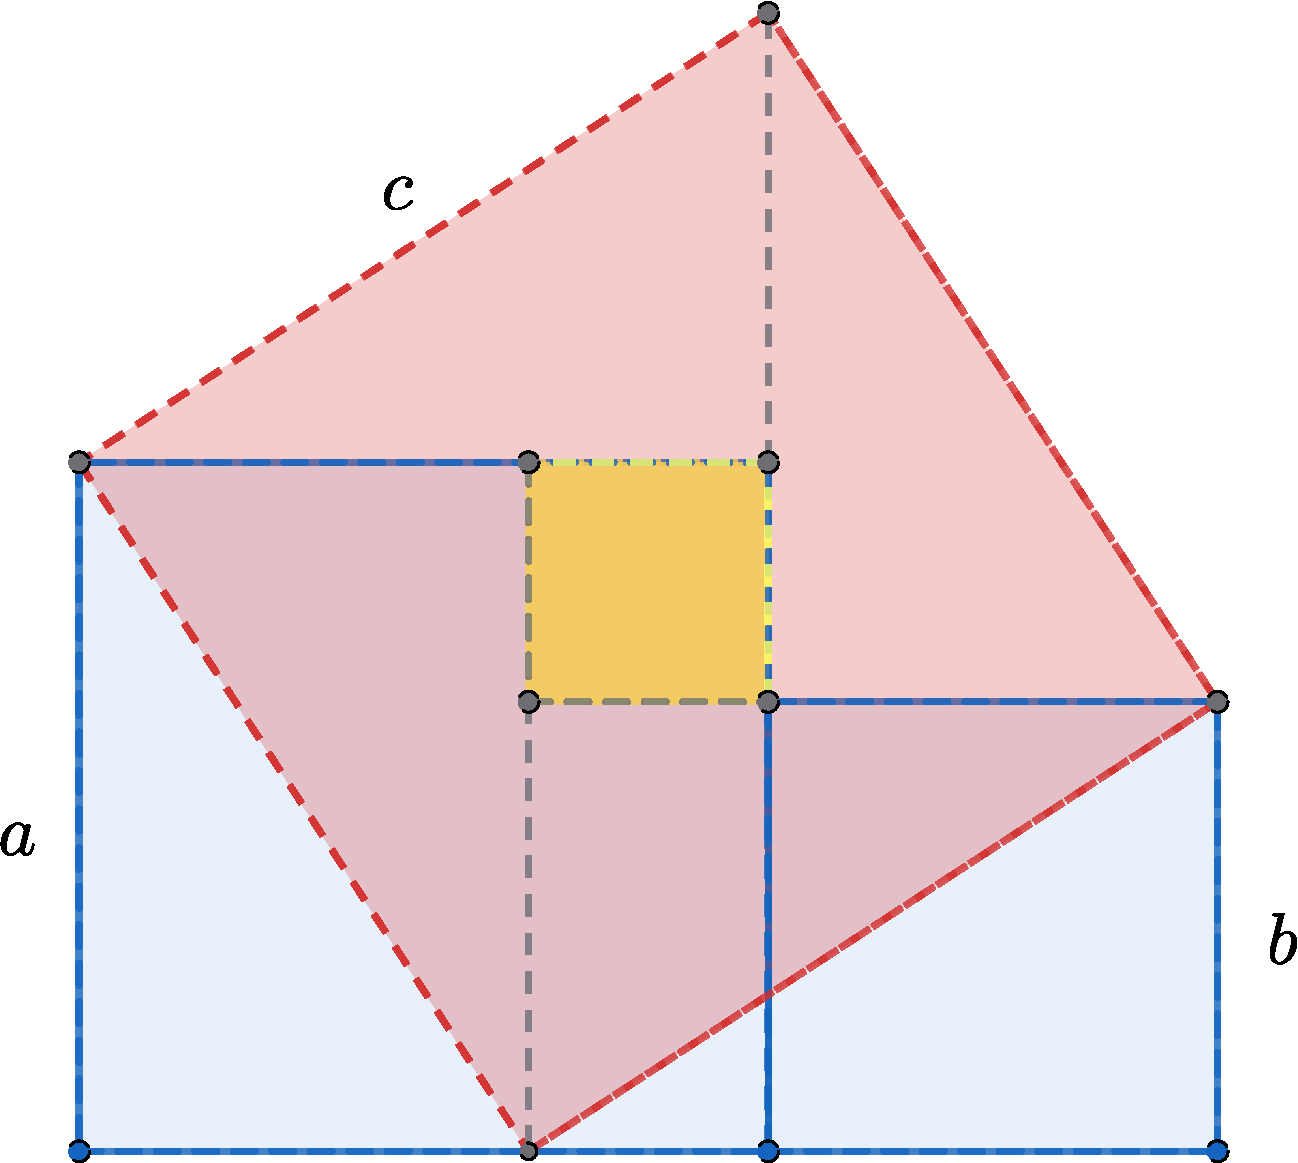
\includegraphics[scale=0.2]{img/zhaoshuang}}
 \caption{赵爽弦图成为了2002年在北京召开的国际数学家大会和中国数学会的会徽。\label{fig:cms-zhaoshuang}}
\end{figure}

这一定理自提出以来,吸引了无数聪明的头脑对它进行证明。如今在中学数学课堂上就至少有“赵爽弦图”(见\cref{fig:cms-zhaoshuang}),传说中的“毕达哥拉斯证法”(见\cref{fig:pythagoras-pww})和《原本》证法。在4000年的时间里,诞生了超过300多种不同的证明,包括意大利文艺复兴时期的全才达芬奇(见\cref{fig:davinci})和美国总统加菲尔德。

\begin{figure}[htbp]
 \centering
 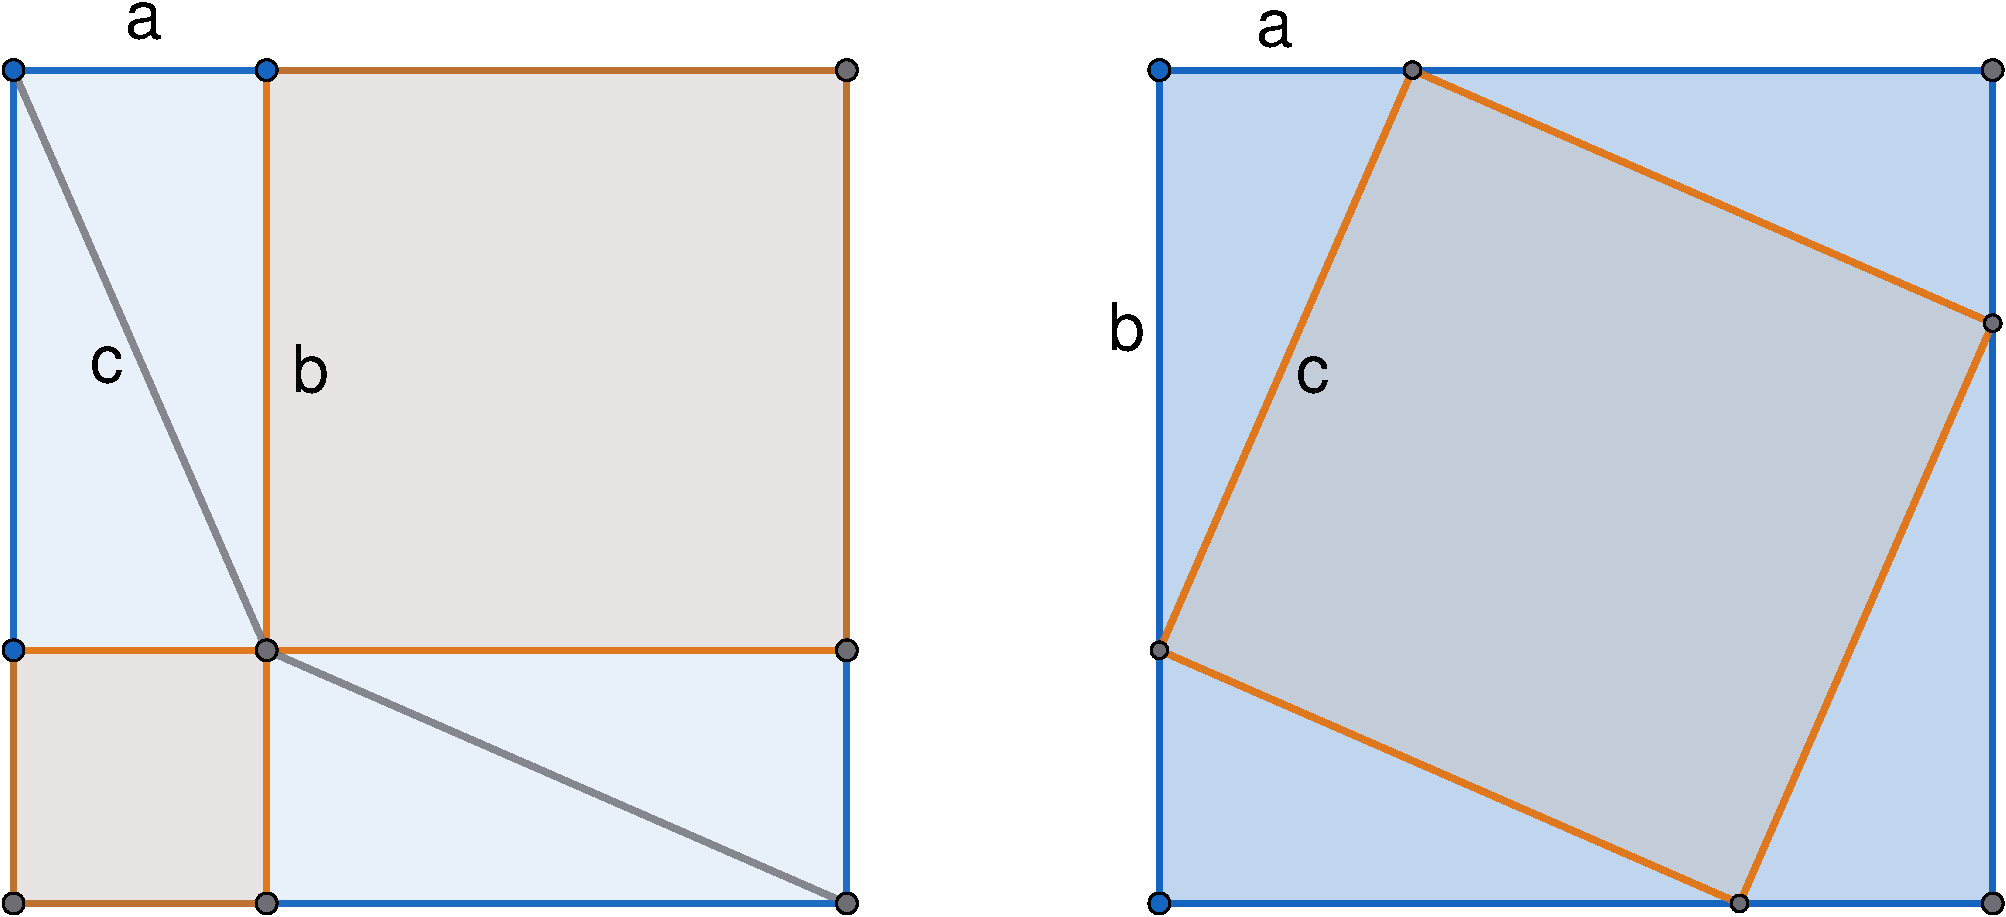
\includegraphics[scale=0.25]{img/pythagoras-pww}
 \caption{传说中的毕达哥拉斯证法\label{fig:pythagoras-pww}}
\end{figure}

达芬奇的方法把原直角三角形复制两份:一份上下颠倒拼到上方,一份平移拼到斜边组成的正方形下方。此时把\cref{fig:davinci}中的“T”形点划线上方的四边形左右镜像翻转,就拼出一个和下方全等的六边形。它们的面积相等,因此各自减去两个原直角三角形的面积后仍相等,即$a^2 + b^2 = c^2$。\cref{qn:pythagoras-thm-garfield}要求解释美国总统加菲尔德的证明方法。

\begin{figure}[htbp]
 \centering
 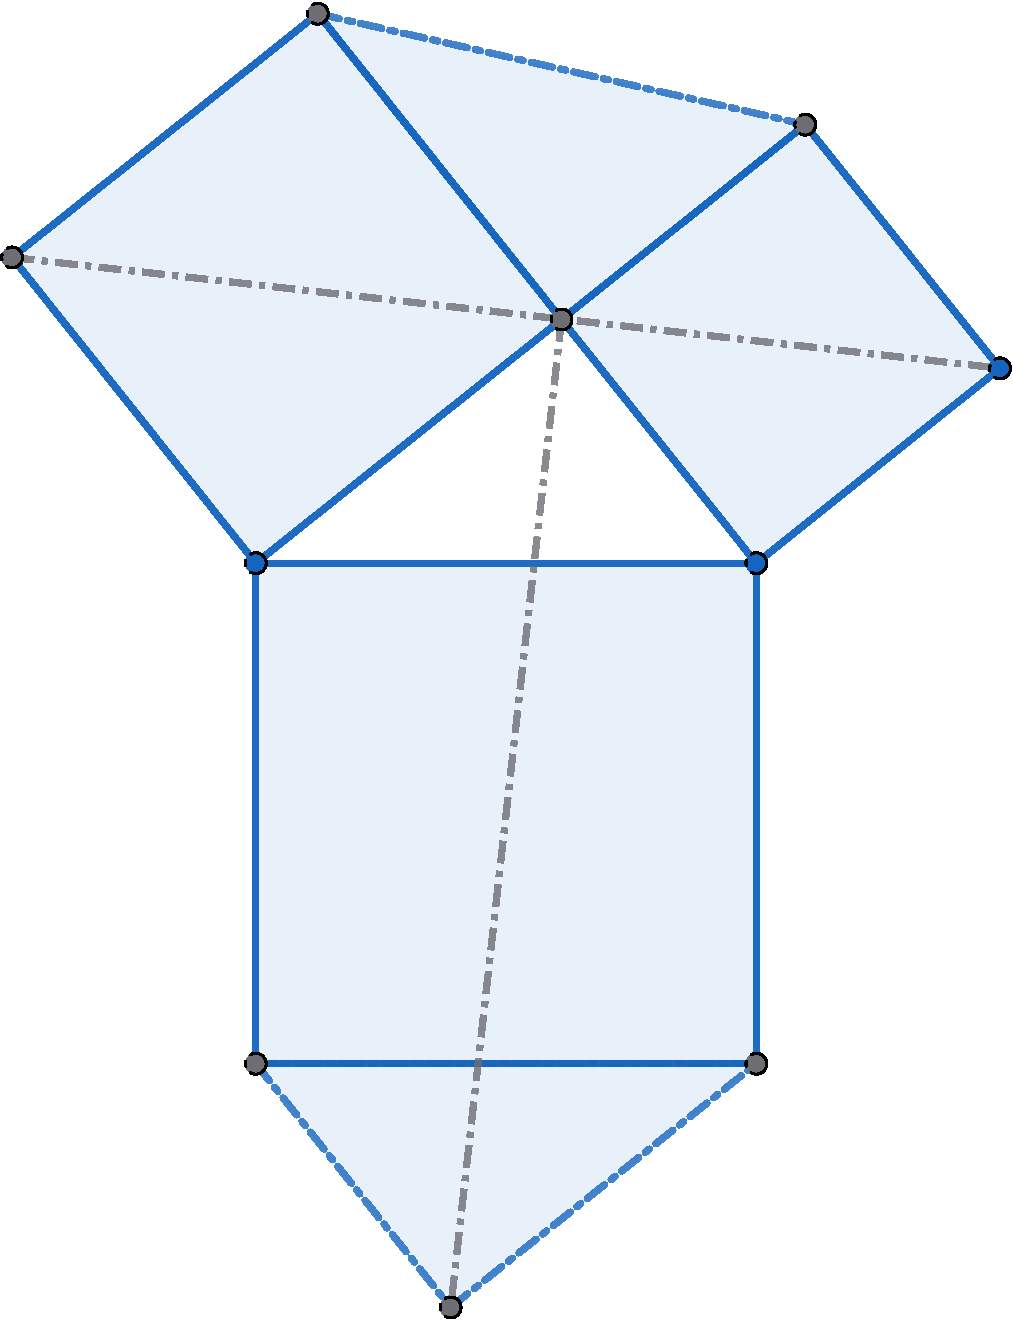
\includegraphics[scale=0.3]{img/davinci}
 \caption{列昂纳多·达·芬奇证法\label{fig:davinci}}
\end{figure}

勾股定理具有非凡的意义,犹如发源的清泉,流淌出了三条壮阔的大河\cite{Stillwell-2010}:1)数论,通过寻找哪些数构成勾股数(也叫做毕达哥拉斯三元组),古希腊人开启了数学皇冠上的明珠——数论的研究。2)几何,勾股定理本身就是一条定量的几何定理。3)无穷,把勾股定理和欧几里得算法结合,古希腊人被无穷次的递归困扰,直接导致了无理数的发现。

\section{数论}
并非任意两个平方数的和一定是平方数,例如$3^2 + 5^2 = 34$不是任何正整数的平方。我们把满足勾股定理的三个正整数$(a, b, c)$叫做勾股数或毕达哥拉斯三元组\footnote{Pythagoras triple}。各个文明都发现了常见的勾股数如$3^2 + 4^2 = 5^2$,$5^2 + 12^2 = 13^2$。古巴比伦的石板上刻有长长的勾股数表。那么究竟怎样找到勾股数?勾股数是有限多还是无限多?这个问题是欧几里得彻底解决的。欧几里得指出,如果$a^2 + b^2 = c^2$成立,那么这组勾股数的倍数也是勾股数,因为:

\begin{align*}
(ka)^2 + (kb)^2 &= k^2(a^2 + b^2) & \text{分配律} \\
  &= k^2c^2 & \text{由}a^2 + b^2 = c^2 \\
  &= (kc)^2
\end{align*}

反过来,如果$a, b$含有公因子$k \ne 1$,则$k$一定也是$c$的因子。同理,如果$b, c$含有公因子$k$,则由于$a^2 = c^2 - b^2$,所以$k$一定也是$a$的因子。本质上我们只需要寻找彼此互素的$a, b, c$(公因子只有1,或$(a, b) = (b, c) = 1$,见\ref{sec:gcd-minus}节),然后乘上倍数就得到更多的勾股数。例如勾股数(12, 16, 20)都是偶数,显然含有公因子2。分别除以2就得到更“简单”的勾股数(6, 8, 10)。继续除以2得到(3, 4, 5)。此时3、4、5彼此互素,已经不能再化简了。我们不妨称这样的勾股数为“最简勾股数”。由于$a$和$a^2$的奇偶相同:奇数的平方还是奇数,偶数的平方还是偶数。如果$a, b$一奇一偶,则$c$一定是奇数。欧几里得进一步排除了$a, b$都是奇数的情况,因为:

\begin{align*}
a^2 + b^2 &= (2m + 1)^2 + (2n + 1)^2 & \text{把}a, b\text{写成奇数形式} \\
  &= 4m^2 + 4m + 1 + 4n^2 + 4n + 1 & \text{分别用完全平方公式展开} \\
  &= 4(m^2 + m + n^2 + n) + 2 = 4k + 2 & \text{令整数} k = m^2 + m + n^2 + n
\end{align*}

这个值除以4余2。但是不管$c$是奇数还是偶数,$c^2$除以4都不可能余2。因为:偶数$(2k)^2 = 4k^2$被4整除,而奇数$(2k + 1)^2 = 4(k^2 + k) + 1$除以4余1。因此$a$和$b$不可能都是奇数,只能是一奇一偶。我们可以任选一个(比如第一个)为偶数,另一个是奇数。这样问题就化简为寻找第一个数为偶数,彼此互素的勾股数。它的答案赫然出现在《几何原本》卷十中的引理1\footnote{《几何原本》中使用正方形代表平方数,并用语言描述做法,见\citepage[330页]{Elements}。这里使用代数符号方便理解。}。

\begin{lemma}[欧几里得《几何原本》卷十,引理1]
方程$x^2 + y^2 = z^2$其中$x, y, z$彼此互素,且$x$是偶数的\underdot{所有}正整数解,可表示为:
\be
\begin{cases}
x = 2mn \\
y = m^2 - n^2 \\
z = m^2 + n^2
\end{cases}
\ee
其中$m > n$,是奇偶不同且互素的任意正整数。
\end{lemma}

注意“所有”二字,这意味着不存在其它最简勾股数能逃出欧几里得的解。换言之,这是\underdot{充分必要}条件。我们接下来证明这一优美的结论。

\begin{proof}
首先正向证明充分性:

\begin{align*}
x^2 + y^2 &= (2mn)^2 + (m^2 - n^2)^2 & \text{代入} \\
  &= 4m^2n^2 + m^4 + n^4 - 2m^2n^2 & \text{完全平方公式展开} \\
  &= m^4 + n^4 + 2m^2n^2 = (m^2 + n^2)^2 &\text{反向用完全平方公式} \\
  &= z^2 &\text{代入}z
\end{align*}

接下来反向证明必要性。把$x^2 + y^2 = z^2$移项后用平方差公式:
\begin{align}
x^2 &= z^2 - y^2 = (z + y)(z - y) &\text{平方差公式} \label{eq:x-as-z-pm-y} \\
(\frac{x}{2})^2 &= (\frac{z + y}{2}) (\frac{z - y}{2}) &\text{左右同除以4}
\end{align}

$x$是偶数,$y, z$都是奇数,故$z \pm y$都是偶数。因此左边的$\frac{x}{2}$,右边的$\frac{z \pm y}{2}$都是正整数。进一步,由于$z, y$互素,所以$\frac{z + y}{2}$和$\frac{z - y}{2}$也互素(见\cref{qn:coprime-of-half-a-pm-b})。如果两个互素的数的乘积是一个平方数,则它们也都是平方数(见\cref{qn:coprime-product-as-square})。因此:

\begin{align*}
\frac{z+y}{2} &= m^2 \\
\frac{z-y}{2} &= n^2
\end{align*}

其中正整数$m > n$。两式相加消去$y$求得$z = m^2 + n^2$,两式相减消去$z$求得$y = m^2 - n^2$。代入\cref{eq:x-as-z-pm-y}得:$x^2 = 2m^2 2n^2$,故$x = 2mn$。
\end{proof}

例如取$m = 2, n = 1$就得到(3, 4, 5),取$m = 3, n = 2$就得到(12, 5, 13)。而所有勾股数的就可以表示为:

\be
x = 2mnr, \quad y = r(m^2 - n^2), \quad z = r(m^2 + n^2)
\ee

其中$r$是任意正整数。

\begin{figure}[htbp]
 \centering
 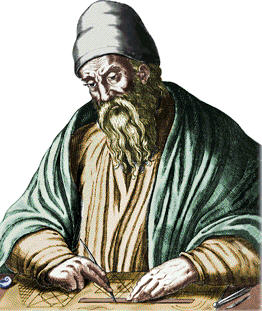
\includegraphics[scale=0.6]{img/Euclid}
 \caption{欧几里得,约公元前300年前后}
 \label{fig:Euclid}
\end{figure}

\begin{mdframed}

\index{欧几里得}
欧几里得(Euclid)是古希腊数学家,以其所著的《几何原本》闻名于世。对于他的生平,现在知道的很少。柏拉图学派晚期的导师普罗克洛斯(Proclus)在《几何学发展概要》中记述了这样的趣事:当时的埃及国王,亚历山大的托勒密一世有一次问欧几里得,学习几何学又没有什么捷径可走。欧几里得回答到:“在几何里,没有专为国王铺设的大道。\footnote{也译为“几何无王者之道”}”(There is no royal road to geometry),学习没有捷径成为了千古传颂的箴言。斯托比亚斯(Stobaeus)记述另一则故事说。一个学生刚开始学习第一个命题,就问欧几里得学习几何后将得到什么。欧几里得说:“给他三个钱币,因为他想在学习中获取实利。”由此可知欧几里得主张学习必须循序渐进、刻苦钻研、不赞成投机取巧的作风,也反对狭隘的实用观点\cite{Elements}。

欧几里得的《几何原本》是一部划时代的著作。其伟大的历史意义在于它是用公理建立起演绎体系的最早典范。过去所积累下来的数学知识是零碎的、片断的,可以比作木石砖瓦。只有借助于逻辑方法,把这些知识组织起来,加以分类比较,解释彼此间的内在联系,整理在一个严密的系统之中,才能建成巍峨的大厦。《几何原本》完成了这一艰巨的任务,它对整个数学的发展产生了深远的影响。

《几何原本》的英文译作The thirteen books of Euclid's elements,直译成中文是欧几里得原本十三卷,简称《原本》(英文简称Elements)。这十三卷包含几何、恒等式、比例论、数论、无理量、穷竭法、正多面体等内容,是古希腊数学的集大成者。明代末年,《原本》前六卷传入中国,学者徐光启和传教士利玛窦与1607年合作将其翻译成中文。可能是因为前六卷集中于几何学(第七到十卷才包含数论),徐光启将其命名为《几何原本》。其中译定的一些重要术语沿用至今。遗憾的是,利玛窦的去世和明清之际的剧变中断了后七卷的翻译工作。直到250年后的1857年,中国数学家李善兰和英国传教士伟烈亚力才将完整的《几何原本》译出。他们以英译本为底本,译出了后九卷,包括被认为是后人添加的第14,15卷。李善兰曾在曾国藩军中效力,他把译稿交给曾国藩说,松江刻本已经毁于战乱了,如果不再出版,这样的绝学就会失传(“此算学家不可少之书,失今不刻,行复绝矣。”)。曾国藩嘱托李善兰把前六卷重新订正,汇集在一起。同治四年(1865年)十月,曾国藩为此书作序,并主持重刻出版。这推动了《几何原本》在近代中国的传播和影响。考虑到这十三卷的内容不仅包含几何,今天在部编版中小学数学教材中,已经统一使用《原本》这个译法。我们也推荐读者朋友们使用《原本》或者《欧几里得原本》这样的叫法。
%% https://www.zhonghuashu.com/wiki/%E5%B9%BE%E4%BD%95%E5%8E%9F%E6%9C%AC/%E5%BA%8F

两千多年来,这部著作在几何教学中一直占据统治地位,在二十世纪初依然用于数学课的基本教材。包括我国在内的许多国家仍将其作为中学的必修科目(现在中学的几何课本是按照法国数学家勒让德《原本》改写本思路编写的),并作为训练逻辑推理的最有力教育手段\cite{HanXueTao16}。
\end{mdframed}

尽管彻底解决了$x^2 + y^2 = z^2$的所有整数解问题,但$x^3 + y^3 = z^3$,$x^4 + y^4 = z^4$,或者更一般的$x^n + y^n = z^n$(其中整数$n \geq 3$)却难住了古人。似乎除了$x = y = z = 0$再也找不出任何整数解了。我们要等到1800年后的十七世纪,青年“业余”数学家费马才在$n = 4$上获得突破(见第6章)。勾股定理的整数解问题展示了数论这一数学分支的典型问题:研究数,特别是整数的性质。在很长一段时间,这门学科被称为“算术”(arithmetic),例如古希腊数学家丢番图的名著《丢番图算术》,德国数学家高斯的化时代著作《算术研究》都是数论方面的经典。奇偶性、素数、整除、公因子,余数等概念是这门学科的基础概念。在“长方形数”的探索中,古希腊人发现某些数可以表示成长方形,如$12 = 3 \times 4$可以用三行四列的小石子摆出。这样就引出了因数的概念,长方形数的边长就是其因子。并且因子可能有多个,例如$12 = 3 \times 4 = 2 \times 6$,所以2、3、4、6都是12的因子。但是有些数却无法表示成长方形数,例如5,只能摆成一行五个石子或一列五个石子\footnote{显然古希腊人在这里区分了线段和矩形,他们并不认可$1 \times 5$或$5 \times 1$是一个长方形数。}。这种数形结合的方法引出了素数的概念。素数$p$只能被1和$p$整除,是构成其它数的砖石。前几个素数是2、3、5、7、11……这样的探索自然引出了有趣的问题:1)作为构成其它数的砖石,素数有多少个?是有限多还是无限多?2)素数的出现有何规律?有没有产生素数的公式和方法?其中第一个问题又是由欧几里得解决的,而埃拉托斯特尼在第二个问题上迈出了关键的第一步。

自从芝诺悖论提出后,古希腊人就试图避免无穷这个概念。亚里士多德认为所有芝诺悖论中的问题都源自无穷,他提出了一个影响至今的区分:潜无穷和实无穷\footnote{英文分别是potential infinity和actual infinity}。所谓潜无穷或潜无限,是指无限在永远延伸着,是一种变化的、不断产生出来概念。它永远在构造中,永远完成不了,是潜在的,而不是实在的。自然数就是一种潜无穷,对于任何一个自然数$n$,我们都可以找到它的后继$n + 1$,也就是一个更大的自然数。欧几里得几何中的直线也是一种潜无穷,我们可以按需延伸直线。所谓实无穷是指把无限的整体本身作为一个实在的单位,是已经构造出来的东西。也就是把无限对象看作可完成的过程或无穷整体。在做了这种区分后,亚里士多德承认存在潜无穷,但是拒绝承认实无穷的概念。他对实无穷的排斥深刻而长远地影响了日后数学的发展\cite{HanXueTao16}。亚里士多德代表了当时古希腊的哲学观点,关于潜无穷和实无穷的概念区分以及争论一直影响至今。纵观《原本》全书,欧几里得从未在其中使用“无穷”或者“无限”一词。尽管如此他还是成功证明了素数有无限多个,并且这一证明被人们认为是历史上最优美的证明证明之一。

\begin{theorem}[欧几里得《原本》第九卷,命题20]
预先给定任意多的素数,则有比它们更多的素数。
\end{theorem}

欧几里得在叙述这个命题时,小心谨慎地避免使用无穷这样的说法。“预先给定……总有更多的……”这种处理经常出现在《原本》中。我们今天往往直接说“存在无穷多的素数”。欧几里得在证明这个命题时,使用了著名的反证法。我们用现代的语言来描述这一证明。

\begin{proof}
假设只存在有限多个素数,$p_1, p_2, \dotsc, p_n$。欧几里得构造一个新数:
\[
p_1 p_2 \dotsm p_n + 1
\]
也就是把这$n$个素数乘起来再加一。这个数要么是素数,要么不是素数。

\begin{itemize}
\item 如果它是素数,明显这个数不等于$p_1$到$p_n$中的任何一个,这就在有限多个素数之外又增加了一个新的素数;
\item 如果这个数不是素数,那么它就存在一个素因子$p$。但是由于$p_1$到$p_n$中的任何一个都不能整除构造的这个数(除不尽余1),所以素数$p$与任何$p_1$到$p_n$中的数都不同,是一个新的素数。
\end{itemize}
所以在任何情况下,我们都可以获得一个新的素数。这与有限个素数的假设矛盾,因此存在无穷多的素数。
\end{proof}

欧几里得用反正法得到了一种“存在性证明”,他证明了存在无穷多的素数,但却没有给出怎样得到这些素数。这在我们今天看来,是很自然的一种处理。然而在十九世纪末二十世纪初却引发了关于数学根本性的争论。迄今为止,人们没有发现任何素数公式。我们不说“计算”出素数”,而只能说寻找素数。一个非常低效的方法是从$2, 3, 4, \dotsc$开始逐一检查每个数$n$是否是素数。根据定义,需要检查$n$是否含有1和$n$之外的其它因子。这需要依次判断$2, 3, \dotsc, n - 1 $是否整除$n$。当然,由于$a \times b = b \times a$,我们可以把这个范围缩小到判断$2, 3, \dotsc, \lfloor \sqrt{n} \rfloor$是否整除$n$,即把上限定为不大于$n$的开平方的整数。这个方法很差,除法的计算量非常大。埃拉托斯特尼给出了一种快速寻找素数的方法,被称为埃拉托斯特尼筛法。首先我们列出从2开始的整数:

\[2, 3, 4, 5, 6, 7, 8, 9, 10, 11, 12, 13, 14, 15, 16, 17, 18, 19, 20, \dotsc \]

2是第一素数。然后从2开始,筛除掉所有2的倍数:

\[2, 3, \cancel{4}, 5, \cancel{6}, 7, \cancel{8}, 9, \cancel{10}, 11, \cancel{12}, 13, \cancel{14}, 15, \cancel{16}, 17, \cancel{18}, 19, \cancel{20}, \dotsc\]


接下来的3就是第一轮筛除后新找到的素数。然后再筛除3的倍数:

\[2, 3, 5, 7, \cancel{9}, 11, 13, \cancel{15}, 17, 19, \cancel{21}, 23, 25, \cancel{27}, 29, \dotsc\]

接下来的5是新找到的素数。然后筛除掉所有5的倍数:

\[2, 3, 5, 7, 11, 13, 17, 19, 23, \cancel{25}, 29, \dotsc\]

每轮筛除后,剩余的第一个数$p$是新找到的素数,接下来的一轮筛除掉所有$p$的倍数。这样不断进行下去。通常在应用埃拉托斯特尼筛法时,我们事先定出一个目标:寻找$n$以内的素数。接下来不断进行筛除,直到把不大于$\sqrt{n}$的所有倍数都筛除为止。\cref{qn:seive-of-eratosthenes-100}要求利用筛法找出100以内的所有素数。

%%算术基本定理放在第6章代数数部分引入

有了因子的概念,毕达哥拉斯学派开始研究这些因子和数的关系。他们发现某些数的所有真因子\footnote{真因子是小于数本身的因子}之和恰好等于这个数本身,于是将其命名为完美数(也叫做完全数),并成功地找到两个。最小的完美数是6,因为6的真因子有1、2、3,而6 = 1 + 2 + 3,下一个是28,其真因子为1、2、4、7、14,并且28 = 1 + 2 + 4 + 7 + 14。毕达哥拉斯学派并非纯粹的学术团体,学派信奉数字神秘主义。他们对完美数如此着迷,认为:“6象征着完满的婚姻以及健康和美丽,因为它的部分是完整的,并且其和等于自身。”中世纪后,更是赋予了完美数宗教意义。人们认为6和28是上帝创造世界时所用的基本数字,因为上帝创造世界花了六天,二十八天则是月亮绕地球一周的日数。真正从数论的角度对完美数进行研究并取得关键进展的还是欧几里得。

\begin{theorem}[欧几里得《原本》卷九,命题36]
如果$2^{n+1}-1$是素数,则$2^n(2^{n+1}-1)$是完美数\footnote{这里用代数符号简化了叙述,《原本》原文为:设从单位起有一些连续二倍起来的连比例数,若所有数之和是素数,则这个和乘最后一个数的乘积将是一个完全数。进行对比,不难看出代数符号的威力。}。
\end{theorem}

\begin{proof}
素数$p = 2^{n+1}-1$只有两个因子$1, p$;$2p$含有四个因子$1, 2, p, 2p$;$4p = 2^2p$含有6个因子$1, 2, 4, p, 2p, 4p$;以此类推$2^n p$含有$2(n+1)$个因子$1, 2, 4, \dotsc, 2^n, p, 2p, 4p, \dotsc, 2^n p$。最后一个不是真因子,剩余的真因子和为:

\begin{align*}
s &= 1 + 2 + \dotsb + 2^n + p + 2p + \dotsb + 2^{n-1}p \\
  &= (1 + 2 + \dotsb + 2^n) + p(1 + 2 + \dotsb + 2^{n-1})
\end{align*}

我们在高中学习过等比数列求和,这里不妨用方程从头推导一下。令:

\be
x = 1 + 2 + 4 + \dotsb + 2^n
\label{eq:sum-of-power2}
\ee

把\cref{eq:sum-of-power2}乘以2:

\be
2x = 2 + 4 + 8 + \dotsb + 2^n + 2^{n+1}
\label{eq:2sum-of-power2}
\ee

\cref{eq:2sum-of-power2}减\cref{eq:sum-of-power2}得:

\begin{align*}
2x - x & = \quad \ \cancel{2} + \cancel{4} + \dotsb + \cancel{2^n} + 2^{n+1} \\
       & - 1 - \cancel{2} - \cancel{4} - \dotsb - \cancel{2^n} \\
  x &= 2^{n+1} - 1
\end{align*}

把这个结果代入真因子和求$s$:

\begin{align*}
s & = 2^{n + 1} - 1 + p(2^n - 1) &&\text{代入}p = 2^{n+1} - 1 \\
  & = p + 2^n p - p = 2^n p = 2^n (2^{n+1} - 1) && \qedhere
\end{align*}
\end{proof}

所以$2^n(2^{n+1}-1)$是完美数。后人把这一形式的完美数称为欧几里得完美数。根据欧几里得的结果,不难看出:1)只要找到更多的形如$2^{n+1} - 1$的素数,就能找到更多的完美数。2)所有欧几里得完美数都是偶数,但完美数一定是偶数吗?很容易验证毕达哥拉斯学派的找到的6和28都是欧几里得完美数:$2^1\times(2^2-1)=2 \times 3 = 6$,$2^2 \times (2^3 - 1) = 4 \times 7 = 28$,分别是$n = 1, n = 2$时的情况。但后面就没有这么幸运了。$2^4 - 1 = 15$不是素数。不过$2^5 - 1 = 31$是素数,所以$2^4 \times 31 = 16 \times 31 = 496$是下一个完美数。但$2^6 - 1 = 63$不是素数,$2^7 - 1 = 127$是素数,所以$2^6 \times 127 = 8128$是完美数。接下来$n = 8, 9, 10, 11, 12$都不是素数,下一个素数是$2^{13}-1 = 8191$。凭借手算验证这个数是素数已经很困难了,其对应的完美数更是巨大到了33550336。欧几里得完美数的增加极其快速,由于古希腊人没有强大的位值制十进制计数系统,寻找更多完美数的研究遇到了困境。而问题2)的难度远非常人想象。数学家欧拉进一步证明了,任何偶完美数必然是欧几里得完美数(见附录\ref{app:even-perfect-number})。古希腊人没有找到任何奇完美数。不仅如此,直到今天也没有发现任何奇完美数。于是人们猜想不存在奇完全数,但迄今为止没有人能证明这个猜想。这成了当今数学中的悬案,吸引了从欧拉到陶哲轩一代又一代数学家对它进行研究。

十七世纪,法国神父梅森和数学家费马通过书信往来继续研究了形如$2^n \pm 1$的素数。费马于1640年给出了一个惊人的“素数公式”:

\be
F_n = 2^{2^n} + 1
\ee

计算不难发现:$F_0 = 2^{2^0} + 1 = 3$是素数,$F_1 = 2^{2^1} + 1 = 5$是素数,$F_2 = 2^{2^2} + 1 = 17$是素数,$F_3 = 2^{2^3} + 1 = 257$是素数,$F_4 = 2^{2^4} + 1 = 65537$还是素数。费马高兴地断言,所有$F_n = 2^{2^n} + 1$都是素数!我们可以想像手工验算65537的难度,并且这个指数的指数“爆炸”速度极为惊人。费马的猜测令人兴奋,因为从未有人发现任何有效的产生素数的公式。今天我们称$F_n$为费马数。但是近一个世纪后,大数学家欧拉于1732年发现:$F_5= 641 \times 6700417$是一个合数。并且从那以后,人们利用手算或计算机验算了$F_5$到$F_{30}$,很不幸它们都是合数。是否$n = 5$以后所有的$F_n$都是合数至今仍然是一个未证明的猜想。故事并未结束,第X节我们将会看到费马数惊人地出现在正多边形尺规作图的背后。

\begin{mdframed}
你也许好奇,欧拉是如何手算找到$F_5$的因子的。这是多么巨大的计算量啊!但欧拉就是欧拉,他可能是通过这一巧妙的方法完成对$F_5$的因子分解的\citepage[27页]{Coxeter2022}\citepage[18页]{Hardy2009}。欧拉重新发现费马的研究成果后,必定对费马大定理$x^n + y^n = z^n$感兴趣。在研究四次方和($n = 4$)时很容易遇到$5^4 + 2^4= 641$。而费马数$F_5 = 2^{2^5} + 1 = 2^{32} + 1$。注意到把$641 = 5^4 + 2^4$乘以$2^{28}$就能凑到$2^{32}$:
\[
641 \times 2^{28} = (5^4 + 2^4)2^{28} = 5^42^{28} + 2^{32} = A
\]

令这个数为$A$。从$A$中减去$5^42^{28}$再加上1就是费马数$F_5$,令$B = 5^42^{28} - 1$,则$F_5 = A - B$。另一方面$641 = 640 + 1 = 5 \times 128 + 1 = 5 \times 2^{7} + 1$。注意到它是$B$的一个因子!我们可以两次用平方差公式对$B$进行因式分解:

\begin{align*}
B = 5^4 2^{28} - 1 &= (5^2 2^{14} + 1)(5^2 2^{14} - 1) && \text{平方差公式} \\
  &= (5^2 2^{14} + 1)(5 \times 2^7 + 1)(5 \times 2^7 - 1) && \text{对第2项用平方差公式} \\
  &= (5^2 2^{14} + 1) \times 641 \times (5 \times 2^7 - 1)
\end{align*}

由于641既整除$A$也整除$B$,所以641整除$A - B = F_5$。这样就证明了费马数$F_5$不是素数。这一年(1732年),欧拉只有25岁。
\end{mdframed}

与费马通信、讨论后,梅森对形如$2^n - 1$的素数进行了大量的计算、验证,并取得了重要的进展。我们不知道如下的结论是来自费马、梅森,还是来自后人:

\begin{proposition}[梅森素数]
如果$n > 1$且$a^n - 1$是素数,则必然有$a = 2$并且$n$是素数。
\end{proposition}

\begin{proof}
可以利用等比数列求和公式证明$a = 2$。考虑下面的等比数列:

\begin{align*}
s  &= 1 + a + a^2 + \dotsb + a^{n-1}  \\
as &= a + a^2 + \dotsb + a^{n-1} + a^n && \text{两边乘以}a \\
as - s &= \cancel{a} + \cancel{a^2} + \dotsb + \cancel{a^{n-1}} + a^n - 1 - \cancel{a} - \cancel{a^2} - \dotsb - \cancel{a^{n-1}} \\
(a - 1)s &= a^n - 1 \\
 s &= \frac{a^n - 1}{a - 1}
\end{align*}

这说明$a - 1$是$a^n - 1$的一个因子\footnote{也可以用函数的方法证明这点:考虑函数$f(x) = x^n - 1$,显然$x = 1$是方程$f(x) = 0$的一个解:$1^n - 1 = 0$。因此$x-1$是$x^n - 1$的因子。},但如果$a^n - 1$是素数,它只有1和自己两个因子。这样必然有$a - 1 = 1$,即:$a = 2$。

我们接下来证明$n$必然是素数。用反证法,假设$2^n - 1$是素数,但$n = ab$不是素数,可以分解为两个大于1的数的积。考虑等比数列的和:
\[
s = 1 + 2^a + (2^a)^2 + (2^a)^3 + \dotsb + (2^a)^{b-1}
\]

其中每项都是前一项的$2^a$倍。两边同时乘以$2^a$再减去原数列,消去除首尾的中间项得:

\[
s = \frac{(2^a)^b - 1}{2^a - 1} = \frac{2^{ab} - 1}{2^a - 1}
\]

这说明$2^a - 1$整除$2^{ab} - 1$。并且根据假设$a > 1$,有$2^a - 1 > 1$。这与$2^n - 1 = 2^{ab} - 1$是素数矛盾。所以$n$必然是素数。
\end{proof}

注意,这一命题的逆命题\underdot{不成立}。$p$是素数时,$2^p - 1$不一定是素数。例如$2^{11} - 1 = 2047 = 23 \times 89$。但这一命题使得梅森只需要寻找形如$2^p - 1$的素数。1644年,梅森在他的著作《物理数学随感》\footnote{拉丁文Cogitata Physica-Mathematica}的前言中断言:在$257$以内,只有$p$等于2, 3, 5, 7, 13, 17, 19, 31, 67, 127, 257时$2^p - 1$才是素数。尽管这一列表有两处错误(有两个不是素数,但缺失了两个真正的素数,正确的列表应为:2, 3, 5, 7, 13, 17, 19, 31, 61, 89, 107, 127)梅森的发现仍然极为重要。今天,人们定义这样的素数为梅森素数,记为$M_p = 2^p - 1$。尽管没有费马数那样“指数的指数级爆炸”,梅森素数依然是“指数爆炸”式增长的,没有人能轻易验证$M_p$是否是素数。直到1750年,欧拉才验证了$M_{31}$的确是素数。但即使是欧拉也错误地断言$M_{41}$和$M_{47}$是素数。人们直到1886年才发现梅森漏掉了$M_{61}$这个素数。1876年,法国数学家卢卡斯发现了一种检验梅森素数的方法,并成功确认了$M_{127}$是素数。这一素数长达39位。同时卢卡斯判定$M_{67}$不是素数,但是他并未找到其因子。1903年数学家科尔在一次数学会议上走上讲台,一言不发在黑板上写下:$2^{67} - 1 = 193707721 \times 761838257287$。面对台下的掌声,科尔说这花掉了了他三年来的每个星期天。今天人们利用计算机和互联网的强大算力寻找更多的梅森素数。截至2024年,人们共发现了52个梅森素数。其中第52个为$2^{136279841} - 1$共有41024320位。这个记录还在不断被打破。

\begin{figure}[htbp]
 \centering
 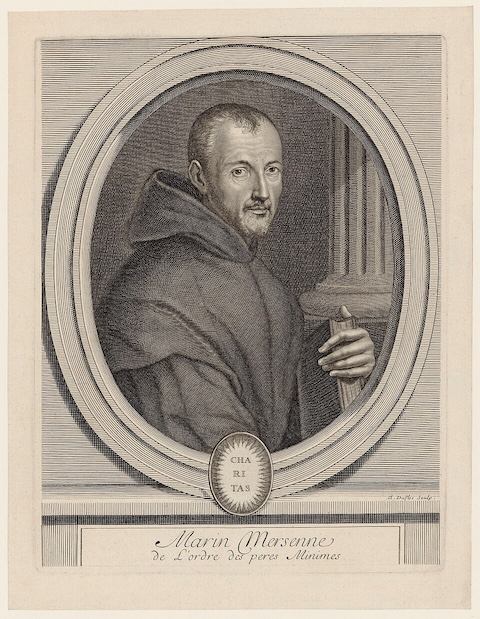
\includegraphics[scale=0.35]{img/MarinMersenne}
 %% https://commons.wikimedia.org/wiki/File:MarinMersenneDuflos.jpg
 \caption{克劳德·迪弗洛创作的版画:马林·梅森像}
 \label{fig:marin-mersenne}
\end{figure}

\begin{mdframed}
马林·梅森(Marin Mersenne, 1588~1648,见\cref{fig:marin-mersenne})是法国著名的修道士、自然哲学家、数学家。他是17世纪欧洲科学界中独特的中心人物。梅森与当时欧洲最伟大的思想家、科学家、数学家保持通信,定期组织学术讨论,发表并传播他们的成果,鼓励年轻的学者参与科学研究,极大地促进了法国和欧洲的科学和思想进步。

%% https://mathshistory.st-andrews.ac.uk/Biographies/Mersenne/
1588年9月8日,梅森生于法国一个普通工人家庭。尽管家庭经济条件不好,父母坚持让他接受教育。16岁时,梅森进入了拉弗莱什新成立的耶稣会学校。这所优秀的学校也招收穷人的子女,从这里走出了梅森和笛卡尔这些优秀的毕业生。1609年他从巴黎的索邦神学院毕业,并于1612年起担任神父。如果我们结合当时的历史背景,就会惊异于梅森如何成为了欧洲先进学术思想的中心人物。这是一件极为困难并且具有生命危险的工作。罗马教廷正在疯狂镇压新思想。哥白尼的《天体运行论》遭到封禁,布鲁诺遭遇火刑,伽利略被迫“认罪”,笛卡尔远走荷兰,帕斯卡假借外省人和索邦的神学家论战\footnotemark。作为神父的梅森却既得到教会的支持,又成为了各国科学家的秘密战友。我们不难想象他超人的沟通能力和受人尊敬的人格。

梅森热爱数学,他认为没有数学就没有科学。从1623年起,梅森小心翼翼地邀请欧洲的顶级学者到他位于巴黎的修道院访问,或者进行通信。有些人甚至远达君士坦丁堡和今天的罗马尼亚。梅森的常客包括佩雷斯克、伽森狄、笛卡尔、罗贝瓦尔、贝克曼、范·海尔蒙特、费马、霍布斯和帕斯卡父子。他每周组织会议,宣读或评议论文,交换学者间的联系方式,讨论实验或研究计划。这个以梅森为中心的小圈子俨然是今天的学术团体,被称为“巴黎学院”。由于梅森是中心人物,也被戏称为“梅森学院”。法国学术界认为,这是后来的法兰西科学院的前身。梅森的学者朋友越来越多,每当收到邀请,他就赶赴他国进行访问。

梅森喜爱音乐,他研究了声学理论和声音传播的速度。1627年他发表了《宇宙的和谐》一书,首次指出弦振动的频率正比于张力的平方根;反比于弦长、直径;反比于弦质量的平方根。梅森善于发现有才华的年轻人,鼓励他们分享想法和成果。年轻的罗贝瓦尔在巴黎的讨论会中崭露头角,梅森很快注意到了他,并建议他研究摆线这一课题。1638年,罗贝瓦尔成功计算出了摆线下的面积。年轻的惠更斯视梅森为榜样。在梅森的鼓舞下,他发表了《音乐的理论》一书。1644年10月,梅森访问了意大利,他了解到了伽利略的学生托里拆利进行的大气压实验(这一实验成功证实了大气是有重量的,大气压可以顶起约76厘米汞柱)。返回巴黎后,他组织学者们进行讨论,帕斯卡进一步通过实验验证了大气压随海拔的变化。可惜梅森没能看到实验结果就病逝了。今天,我们用帕斯卡作为国际压强单位以纪念这一研究。梅森几乎把他的一生献给了科学。1648年9月1日,梅森病逝于巴黎,他要求把自己的遗体用于生物学研究\cite{OConnor-Robertson-2005}。

%% https://www.britannica.com/biography/Marin-Mersenne
梅森的一些工作意义重大却极有风险。他帮助隐居于荷兰的笛卡尔出版了《谈谈方法》一书(被教会列为禁书),收集了主要学者对于笛卡尔《第一哲学沉思集》的反驳意见。在教会封禁的情况下坚持在法国出版了伽利略的著作,促进了新学术思想在欧洲的传播\cite{Britannia-2024}。梅森死后,人们从他的住所整理出了78位学者间的通信,包括费马、惠更斯、佩尔、伽利略、托里拆利等人,若干科学仪器以及大量书籍。这些文献后来被集结出版,成为了17世纪科学研究的宝贵财富。
\end{mdframed}
\footnotetext{见帕斯卡《致外省人信札》}

\section{无理数}
勾股定理(毕达哥拉斯定理)是一把双刃剑。一方面,它在几何、数论、分析等方向上产生了丰富的成果,另一方面它反过来攻击了毕达哥拉斯学派“万物皆数”的信念。与我们今天的概念不同,毕达哥拉斯学派的“数”指整数或者整数的比。所谓万物皆数是相信世间万物都可以表示为这样的数。如果自然界中存在某个量,但却不能表示成整数的比,那么毕达哥拉斯学派的根基就崩塌了。而勾股定理就是寻找这样的数的钥匙。由于这样的数不容于学派的哲学理念,所以被称为“无理数”,而整数或整数的比被称为“有理数”。整数与分数都是有理数,记为$\mathbb{Q}$,对应的英文是Quotient(商)。读者朋友们也许会问:有理数的英文是Rational numbers,为什么不用$\mathbb{R}$来表示有理数呢?这是因为字母$\mathbb{R}$被用来表示实数(英文Real numbers,见XX节),为了加以区分,数学家最终选用了$\mathbb{Q}$作为有理数的符号。它也的确更好地反映了有理数的本质属性(分数可表示为商,整数可表示成除数为1的商)。

古希腊\underdot{传说}希帕索斯(Hippasus)发现了无理数。这则故事为人们津津乐道,被说得有模有样。约公元前470年左右,毕达哥拉斯学派的学生希帕索思试图寻找正方形的对角线所代表的数。可是根据毕达哥拉斯定理,希帕索斯无论如何也找不到一个整数比能够等于正方形的对角线。他把这个发现告知学派的其他人,这造成了极大的恐慌。学派认为这将动摇他们在学术界的统治地位,于是极力封锁该真理的流传。希伯索斯被迫流亡他乡。不幸的是,他最终被毕达哥拉斯学派的门徒困在一条船上,并被沉入大海灭口。这则传说还有另外一个版本。毕达哥拉斯学派用五角星作为徽章和联络标志。希帕索思从神秘五角星标志上得到了启发。如果在边长为1的正五边形内画一个五角星,他发现五角星的对角线长度无法表示成整数的比,从而发现了无理数。这则传说反映了毕达哥拉斯学派的另一面:这个数字神秘主义团体更像是一个“兄弟会”。还有一则故事说,学派的一个成员流落异乡,贫病交迫,无力酬谢房主的款待,临终前要房主在门上画一个五角星。若干年后,有同派的人看到这个标志,询问事情的经过,厚报房主而去\cite{HanXueTao16}。美国迪士尼在1959年的动画片《唐老鸭漫游数学奇境》中,描绘了唐老鸭遇到了毕达哥拉斯和他的朋友们,在了解音乐、艺术与数的关系后,唐老鸭的手掌上也画上了神秘的五角星。

\begin{figure}[htbp]
 \centering
 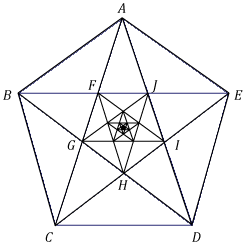
\includegraphics[scale=0.5]{img/pentagram}
 \caption{递归的五角星}
 \label{fig:pentagram}
\end{figure}

可是希帕索斯的传说经不起推敲,没有任何古代文献记录了这一事件。唯一与希帕索斯相关的说法来自亚里士多德,说希帕索斯与赫拉克利特都认为火是宇宙中的第一元素。毕达哥拉斯学派用五角星作为学派徽章,人们在用尺规绘制这一徽章的时候,能够轻易发现正五边形与正五角星相互嵌套以至无穷的特点(见\cref{fig:pentagram})。这些追寻宇宙奥秘的学者们不可能对此感到害怕和恐慌,而是感到好奇和着迷。说希帕索斯发现$\sqrt{2}$也很可疑,等腰直角三角形如此特殊,任何了解勾股定理的人都会发现这个特殊的值。根据亚里士多德的说法,毕达哥拉斯学派用归谬法(即反证法)证明了$\sqrt{2}$的无理性:

\begin{theorem}[毕达哥拉斯]
$\sqrt{2}$不能表示为整数的比,它是无理数。
\end{theorem}

\begin{figure}[htbp]
  \centering
  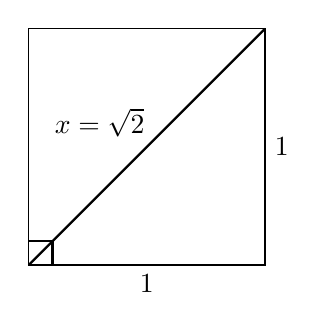
\begin{tikzpicture}[scale=3]
    \draw (0,0) -- (1,0) -- (1,1) -- (0,1) -- cycle;
    \draw[thick] (0,0) -- (1,1);
    \node[below] at (0.5,0) {$1$};
    \node[right] at (1,0.5) {$1$};
    \node[above, sloped] at (0.3,0.5) {$x = \sqrt{2}$};
    \draw[thick] (0.1,0) -- (0.1,0.1) -- (0,0.1);
  \end{tikzpicture}
  \caption{边长为1的正方形和对角线}
  \label{fig:square-diagonal}
\end{figure}

这一定理曾经以命题117出现在欧几里得《原本》卷十中。对比古代的版本,人们发现它是后人加入的。最新的《原本》已经删除了此定理。考虑边长为1的正方形和对角线(间\cref{fig:square-diagonal})。令对角线长为$x$,根据勾股定理有:$x^2 = 1^2 + 1^2 = 2$。记$x = \sqrt{2}$。我们这里给出两种证明方法,其中第一个证明来自毕达哥拉斯。

\begin{proof}
用反证法,假设$x$可以表示为即约分数$\frac{a}{b}$,其中$a, b$互素,且$b \ne 1$。我们有:
\begin{align*}
2 &= x^2 = (\frac{a}{b})^2  && \text{勾股定理} \\
a^2 &= 2b^2  && \text{两边乘以}b^2
\end{align*}
这说明$a^2$是偶数,所以$a$是偶数。令$a = 2c$,代入后得:
\begin{align*}
(2c)^2 &= 2b^2 \\
2c^2 &= b^2 && \text{两边除以}2
\end{align*}
这说明$b^2$也是偶数,因此$b$也是偶数。这与$a, b$互素矛盾。所以$x = \sqrt{2}$无法表示成即约分数,是无理数。
\end{proof}

第二个证明更加一般,它是寻找更多无理数的钥匙:
\begin{proof}
根据$a^2 = 2b^2$,并且$a, b$互素,一定有$b$整除$a^2$。因此$b$的任何素因子$p$也整除$a^2$。因为$p$是素数,所以$p$也整除$a$。这样$p$就既整除$a$也整除$b$,这与$a, b$互素矛盾。
\end{proof}

仔细观察这两个证明就会发现,毕达哥拉斯的证明实际是第二个证明的特殊情况:$p = 2$。下面我们就证明一个更强的定理:

\begin{theorem}
如果$n$不是某个整数的$m$次方,则$\sqrt[m]{n}$是无理数。
\end{theorem}

\begin{proof}
用反证法,假设$\sqrt[m]{n} = \frac{a}{b}$可以表示为即约分数,其中$a, b$互素,且$b \ne 1$。两边乘$m$次方得:
\[
a^m = n b^m
\]
这说明$b$整除$a^m$。因此$b$的任何素因子$p$一定也整除$a^m$。因为$p$是素数,所以$p$也整除$a$。这样$p$就既整除$a$也整除$b$,这与$a, b$互素矛盾。
\end{proof}

作为这个定理的特殊情况,如果$n$不是完全平方数,那么$\sqrt{n}$必然是无理数。这样古希腊人就通过几何量发现了无理数。谈到古希腊几何就一定会谈到尺规作图。顾名思义,就是只用直尺和圆规作图。按照古希腊哲学家柏拉图立下的传统,直尺是没有刻度的。所以其对应的英文是straight edge而非ruler。圆规一旦从平面上抬起,两脚就在重力的作用下自然合拢。这和我们今天使用的文具圆规有所不同。据说这样简陋的绘图工具源自古埃及的拉绳测量。把两点间的绳子绷直相当于画线段,后来演变成了直尺。把绳子的一段固定于某点,取定长的另一端自由移动相当于画圆,后来演变成了圆规。这看来简陋的绘图工具,在严格的规则限制下,却挑战着古希腊学者们的智慧,结出了欧几里得几何学的硕果。文艺复兴时代的伟大艺术家拉斐尔在他的旷世杰作《雅典学院》中描绘了专注用圆规作图的欧几里得(见\cref{fig:euclid-soa})。

\begin{figure}[htbp]
 \centering
 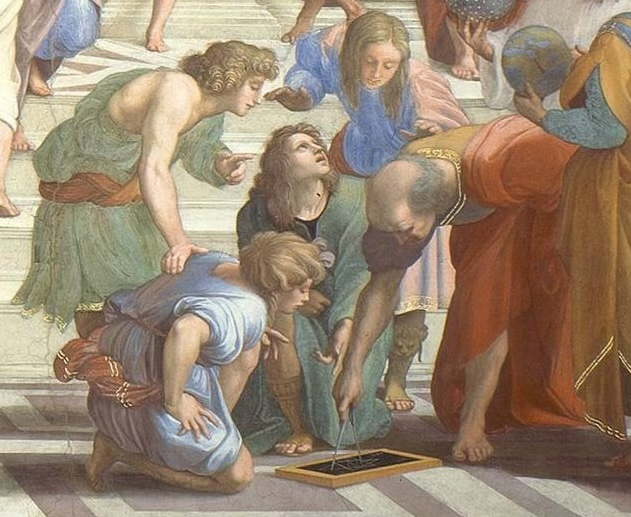
\includegraphics[scale=0.35]{img/euclid-soa}
 \caption{拉斐尔《雅典学院》局部,湿壁画,位于梵蒂冈签字厅}
 \label{fig:euclid-soa}
\end{figure}

在《原本》中,欧几里得甚至把尺规作图以公设确定下来:
\begin{enumerate}[(公设1)]
\item 过两点可作一条直线。(直尺)
\item 一条有限的直线可继续延长。(直尺)
\item 以任意点为心及任意的距离可以画圆。(圆规)
\end{enumerate}

从$\sqrt{2}$开始,古希腊人利用尺规作图和勾股定理(毕达哥拉斯定理)找出了一系列无理数。任给一条线段$AB$,规定其长度为1,用圆规在直线上依次截取长为$AB$的线段$n$次就得到了长为$n$的线段。然后在其一端作垂线(见\cref{qn:perp-of-point}),并截取出长为$m$的线段。最后连接两条相互垂直的线段端点,就得到了直角三角形。根据勾股定理,斜边长度为$\sqrt{n^2 + m^2}$(见\cref{fig:rt-mn})。当$m = n = 1$时,古希腊人就作出了$\sqrt{2}$,当$m=1, n=2$时,古希腊人就作出了$\sqrt{5}$。

\begin{figure}[htbp]
  \centering
  \subcaptionbox{直角边为$n$和$m$的三角形\label{fig:rt-mn}}{
    \begin{tikzpicture}[scale=0.8]
      \draw (0,0) -- (7,0) -- (0,4) -- cycle;
      \node[below] at (3.5,0) {$n$};
      \node[left]  at (0,2) {$m$};
      \node[above, sloped] at (3.5,2.5) {$\sqrt{m^2 + n^2}$};
      \draw[thick] (0.1,0) -- (0.1,0.1) -- (0,0.1);
    \end{tikzpicture}
  }\subcaptionbox{直角边为1和2的三角形\label{fig:rt-12}}{
    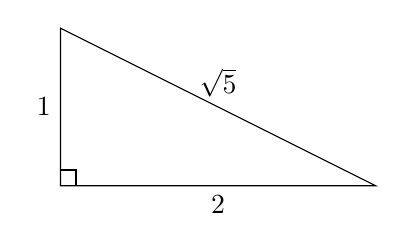
\begin{tikzpicture}[scale=2]
      \draw (0,0) -- (2,0) -- (0,1) -- cycle;
      \node[below] at (1,0) {$2$};
      \node[left]  at (0,0.5) {$1$};
      \node[above, sloped] at (1,0.5) {$\sqrt{5}$};
      \draw[thick] (0.1,0) -- (0.1,0.1) -- (0,0.1);
    \end{tikzpicture}
  }
  \caption{利用勾股定理获得无理数}
  \label{fig:irrational-tagent}
\end{figure}

这个值可不一般。我们延长$\sqrt{5}$一个单位(用圆规在斜边延长线上截取1)得到$1 + \sqrt{5}$,然后再取其一半(见\cref{qn:perp-of-point})得到$\phi = \frac{1 + \sqrt{5}}{2}$。这个值就是大名鼎鼎的黄金分割比。其十进制小数约为1.618\footnote{也叫做黄金分割数、黄金数或黄金比。中学数学课上给出的黄金比近似值是0.618,可以通过在斜边$\sqrt{5}$上截掉1,然后折半得到。}。\cref{fig:gold-ratio}是文艺复兴时期的大师达·芬奇的名作维特鲁威人。据说他正是通过研究完美的人体比例深刻认识到了黄金分割比,并且有意识地在艺术作品的构图和建筑设计中大量使用黄金比。令维特鲁威人的身高为1,腰部以下的部分为$x$,腰部以上为$1 - x$。达·芬奇认识到腰部将人体分割为两部分的比例(即$(1 - x) : x$)等于腰部以下部分与人体身高的比例(即$x : 1$),写成等式就是$(1 - x) : x = x : 1$。欧几里得在《原本》中称其为“极端与平均比率”(extreme and mean ratio)。利用比例内项积等于外项积(见第\ref{sec:frac-equiv}节)将此化为$x^2 + x - 1 = 0$,解二次方程得$x_{1, 2} = \frac{-1 \pm \sqrt{5}}{2}$。

\begin{figure}[htbp]
 \centering
 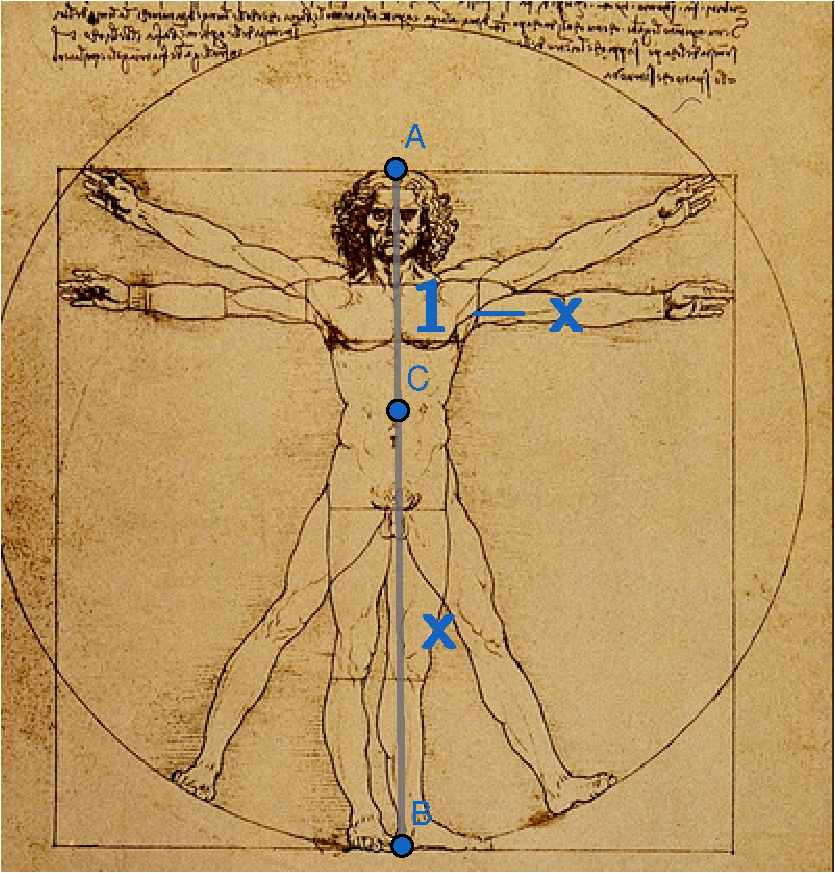
\includegraphics[scale=0.4]{img/gold-ratio}
 \caption{达·芬奇的素描维特鲁威人,1490年}
 \label{fig:gold-ratio}
\end{figure}

由于\cref{fig:gold-ratio}中的$x < 1$,故取$x = \frac{\sqrt{5} - 1}{2} \approx 0.618$。如果令腰部以上的部分为1,腰部以下部分为$x$。同样的黄金分割——使得腰部将人体分割为两部分的比例(即$1 : x$)等于腰部以下部分与人体身高的比例(即$x : (1 + x)$),写成等式就是$1 : x = x : (1 + x)$。这导致另一个方程$x^2 - x - 1 = 0$,解此二次方程得$x_{1, 2} = \frac{1 \pm \sqrt{5}}{2}$。这里由于$x > 0$,故取$x = \frac{1 + \sqrt{5}}{2} \approx 1.618$。注意到这两个值互为倒数:

\[
\frac{\sqrt{5} - 1}{2} \times \frac{\sqrt{5} + 1}{2} = \frac{(\sqrt{5})^2 - 1}{4} = \frac{5 - 1}{4} = 1
\]

所以我们在提到黄金比时,$\phi = \frac{\sqrt{5} \pm 1}{2}$都正确,要取决于上下文的具体含义(见\cref{fig:2-cases-phi})。我们接下来证明黄金数是一个无理数。

\begin{figure}
  \centering
  \subcaptionbox{$\phi = \frac{\sqrt{5} - 1}{2} \approx 0.618$}{
    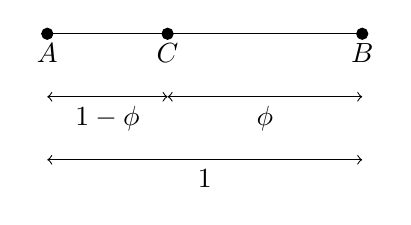
\begin{tikzpicture}[scale=4]
        \pgfmathsetmacro{\a}{0.382}

        \draw (0,0) -- (1,0);

        \filldraw (0,0) circle (0.5pt) node[below] {$A$};
        \filldraw (\a,0) circle (0.5pt) node[below] {$C$};
        \filldraw (1,0) circle (0.5pt) node[below] {$B$};

        \draw[<->] (0,-0.2) -- (\a,-0.2) node[midway,below] {$1-\phi$};
        \draw[<->] (\a,-0.2) -- (1,-0.2) node[midway,below] {$\phi$};
        \draw[<->] (0,-0.4) -- (1,-0.4) node[midway,below] {$1$};
    \end{tikzpicture}
  }\subcaptionbox{$\phi = \frac{\sqrt{5} + 1}{2} \approx 1.618$}{
    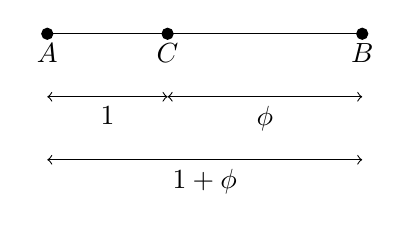
\begin{tikzpicture}[scale=4]
        \pgfmathsetmacro{\a}{0.382}

        \draw (0,0) -- (1,0);

        \filldraw (0,0) circle (0.5pt) node[below] {$A$};
        \filldraw (\a,0) circle (0.5pt) node[below] {$C$};
        \filldraw (1,0) circle (0.5pt) node[below] {$B$};

        \draw[<->] (0,-0.2) -- (\a,-0.2) node[midway,below] {$1$};
        \draw[<->] (\a,-0.2) -- (1,-0.2) node[midway,below] {$\phi$};
        \draw[<->] (0,-0.4) -- (1,-0.4) node[midway,below] {$1 + \phi$};
    \end{tikzpicture}
  }
  \caption{黄金分割的两种含义}
  \label{fig:2-cases-phi}
\end{figure}


\begin{proof}
用反证法,假设黄金数$\phi = \frac{a}{b}$可以写成即约分数,其中$b \ne 1$。它满足方程$\phi^2 \pm \phi - 1 = 0$,代入$\frac{a}{b}$:
\begin{align*}
(\frac{a}{b})^2 & = 1 \pm \frac{a}{b}  \\
a^2 &= b^2 \pm ab && \text{两边乘以}b^2 \\
a^2 &= b(b \pm a)
\end{align*}
因为$a, b$互素,它们不可能都是偶数。如果$a$是奇数$b$是偶数,则左边$a^2$是奇数,但右边是偶数导致矛盾;如果$a$是偶数$b$是奇数,则左边$a^2$是偶数,但右边的$b \pm a$是奇数,乘以奇数$b$还是奇数,也导致矛盾;如果$a, b$都是奇数,则左边$a^2$是奇数,但右边$b \pm a$是偶数,所以右边的值是偶数,仍然矛盾。故假设错误,黄金数是无理数。
\end{proof}

还记得希帕索斯传说的另一个版本么?毕达哥拉斯学派的五角星徽章标志包含着无理数。这个无理数恰好就是黄金分割数$\phi$。我们接下来揭示这个神秘的联系。这一方法来自洛克哈特的《度量》一书。

\begin{figure}[htbp]
 \centering
 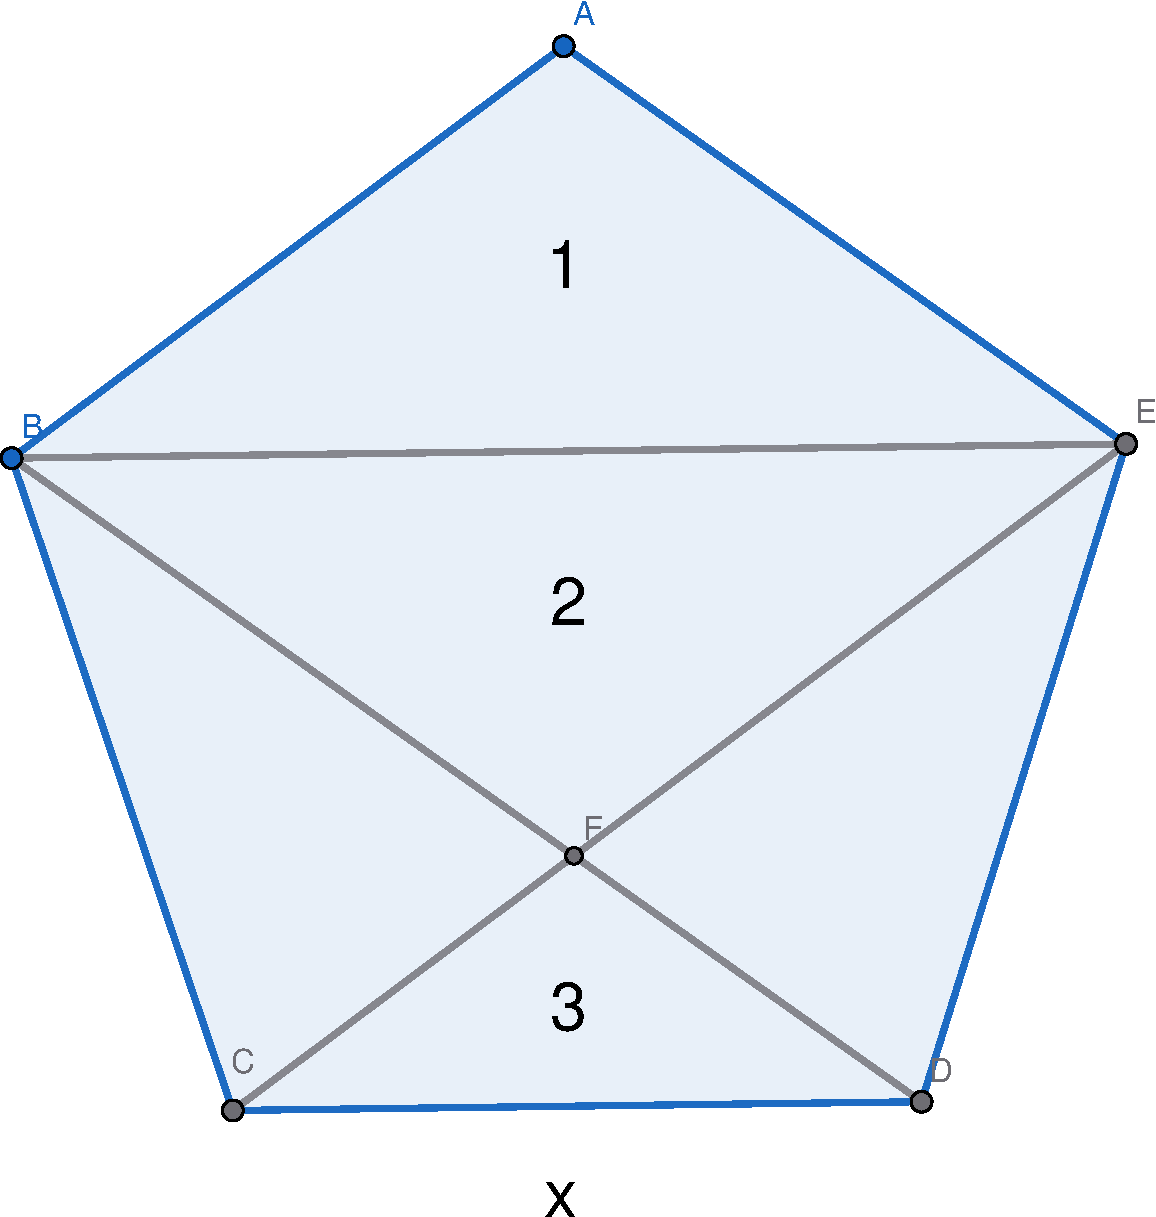
\includegraphics[scale=0.35]{img/pentagon}
 \caption{正五边形}
 \label{fig:pentagon}
\end{figure}

观察\cref{fig:pentagon}中的正五边形,三角形1和2全等,2和3相似(我们略去了详细的证明,不难看出1、2都是等腰三角形,有一公共边,底角都是36度。2、3是有对顶角的等腰三角形)。令对角线$BE$的长度为1,正五边形的边长为$x$,由于三角形1和3相似,所以:

\begin{align*}
\frac{x}{1} &= \frac{AB}{BE} = \frac{FC}{CD} && \text{1, 3相似} \\
            &= \frac{EC - EF}{CD} = \frac{BE - AB}{CD} && BEC\text{是等腰三角形且1, 2全等} \\
            &= \frac{1-x}{x}
\end{align*}

这样就得到方程$x^2 + x - 1 = 0$,它的解恰恰就是黄金分割比$\phi = \frac{\sqrt{5} - 1}{2}$。在毕达哥拉斯学派的徽标中,若五角星的对角线长1,则五角星的邻角距离是$\phi$,五角星的每个角的边长是$1 - \phi$。

Golden ration and Fibonacci series.

\section{欧几里得算法}
Euclidean algorithm,
It's extension and Bezout identity.
Geometric meaning of Euclidean algorithm.
Continue fraction and Euclidean algorithm.
Uncommensurable and irrational numbers, (Elements)

\section{更多的无理数}
Compass and ruler construction II,

polygon construction (pentagon, 17-gon)

Solving polygon construction with number theory, Fermat numbers, Perfect numbers, and Wantzel theorem.

\section{圆周率}
pi as an irrational number

\section{思想之剑}
Dedekind cut

\begin{Exercise}[label={ex:irrationals}]
\Question{正五边形数}
\Question{\cref{fig:garfield}是第20任美国加菲尔德的勾股定理证法,请解释这一证明。\label{qn:pythagoras-thm-garfield}
\begin{center}
 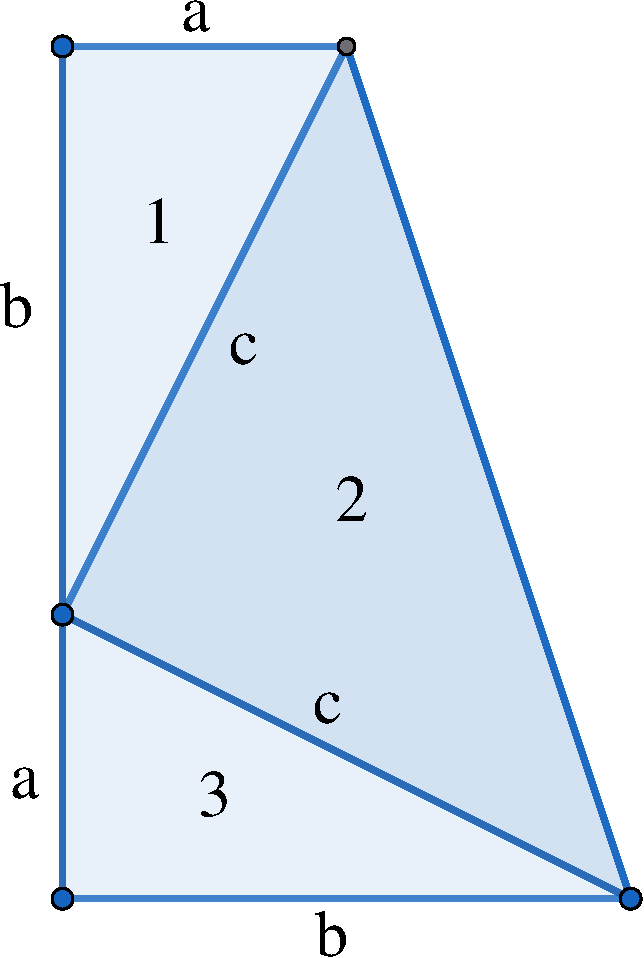
\includegraphics[scale=0.3]{img/garfield}
 \captionof{figure}{美国总统詹姆斯·加菲尔德证法(1876)}
 \label{fig:garfield}
\end{center}
}
\Question{$a, b$是互素的奇数,证明$\frac{a \pm b}{2}$互素。\label{qn:coprime-of-half-a-pm-b}}
\Question{数论中的\underdot{算术基本定理}说:任何整数可以表示成素数的积,不考虑顺序的情况下,这种表示是唯一的。使用算术基本定理证明:$a, b$互素,若$ab = c^2$,则$a, b$都是平方数。\label{qn:coprime-product-as-square}}
\Question{利用埃拉托斯特尼筛法找出100以内的所有素数。\label{qn:seive-of-eratosthenes-100}}
\Question{古希腊的圆规抬起后两脚合拢,无法像今天的圆规那样直接截取线段。在古希腊,给定一条线段$AB$和一条直线$l$,如何在$l$上截取长度$AB$?}
\Question{任给一条线段$AB$,(1) 作其通过$A$点的垂线。(2) 作通过不在$AB$上的一点$C$的垂线。\label{qn:perp-of-point}}
\end{Exercise}

\begin{Answer}[ref={ex:irrationals}]
\Question{正五边形数}
\Question{梯形面积等于两个原直角三角形和一个等腰直角三角形的面积和
}
\Question{%%$a, b$是互素的奇数,证明$\frac{a \pm b}{2}$互素。
  \begin{proof}
    设$d$为$\frac{a \pm b}{2}$的公因子,令$dm = \frac{a + b}{2}, dn = \frac{a - b}{2}$,其中$m, n$为整数。两式相加求得$a = dm + dn = d(m + n)$,所以$d$整除$a$;两式相减得$b = dm - dn = d (m - n)$,所以$d$也整除$b$。这样$d$也是$a, b$的公因子。但$a, b$互素,所以$d$只能是1,即$\frac{a \pm b}{2}$互素。
  \end{proof}
}
\Question{%%$a, b$互素,若$ab = c^2$证明$a, b$都是平方数。
  \begin{proof}
    利用算术基本定理,把$a, b$各自表示为素数幂的积:$a = p_1^{a_1} p_2^{a_2} \dotsm p_n^{a_n}, b = q_1^{b_1} q_2^{b_2} \dotsm q_m^{b_m}$,其中$p_i, q_j$都是素数。由于$a, b$互素,它们的公因数只有1,故$p_i \ne q_j$。它们的积是个平方数$c^2 = p_1^{a_1} p_2^{a_2} \dotsm p_n^{a_n} q_1^{b_1} q_2^{b_2} \dotsm q_m^{b_m}$,所以必然有$a_i, b_j$全部是偶数,即$a, b$都是平方数。
  \end{proof}
}

\Question{%%利用埃拉托斯特尼筛法找出100以内的所有素数。
}

\Question{古希腊的圆规抬起后两脚合拢,无法像今天的圆规那样直接截取线段。在古希腊,给定一条线段$AB$和一条直线$l$,如何在$l$上截取长度$AB$?}

\Question{%%任给一条线段$AB$,(1) 作其通过$A$点的垂线。(2) 作通过不在$AB$上的一点$C$的垂线。

如\cref{fig:perp-of-point}所示,反向延长$AB$,以$A$为圆心$AB$为半径交延长线于点$B'$。分别以点$B$和$B'$为圆心,$BB'$为半径画两圆。连接两圆交点得垂线$CD$。
\begin{center}
 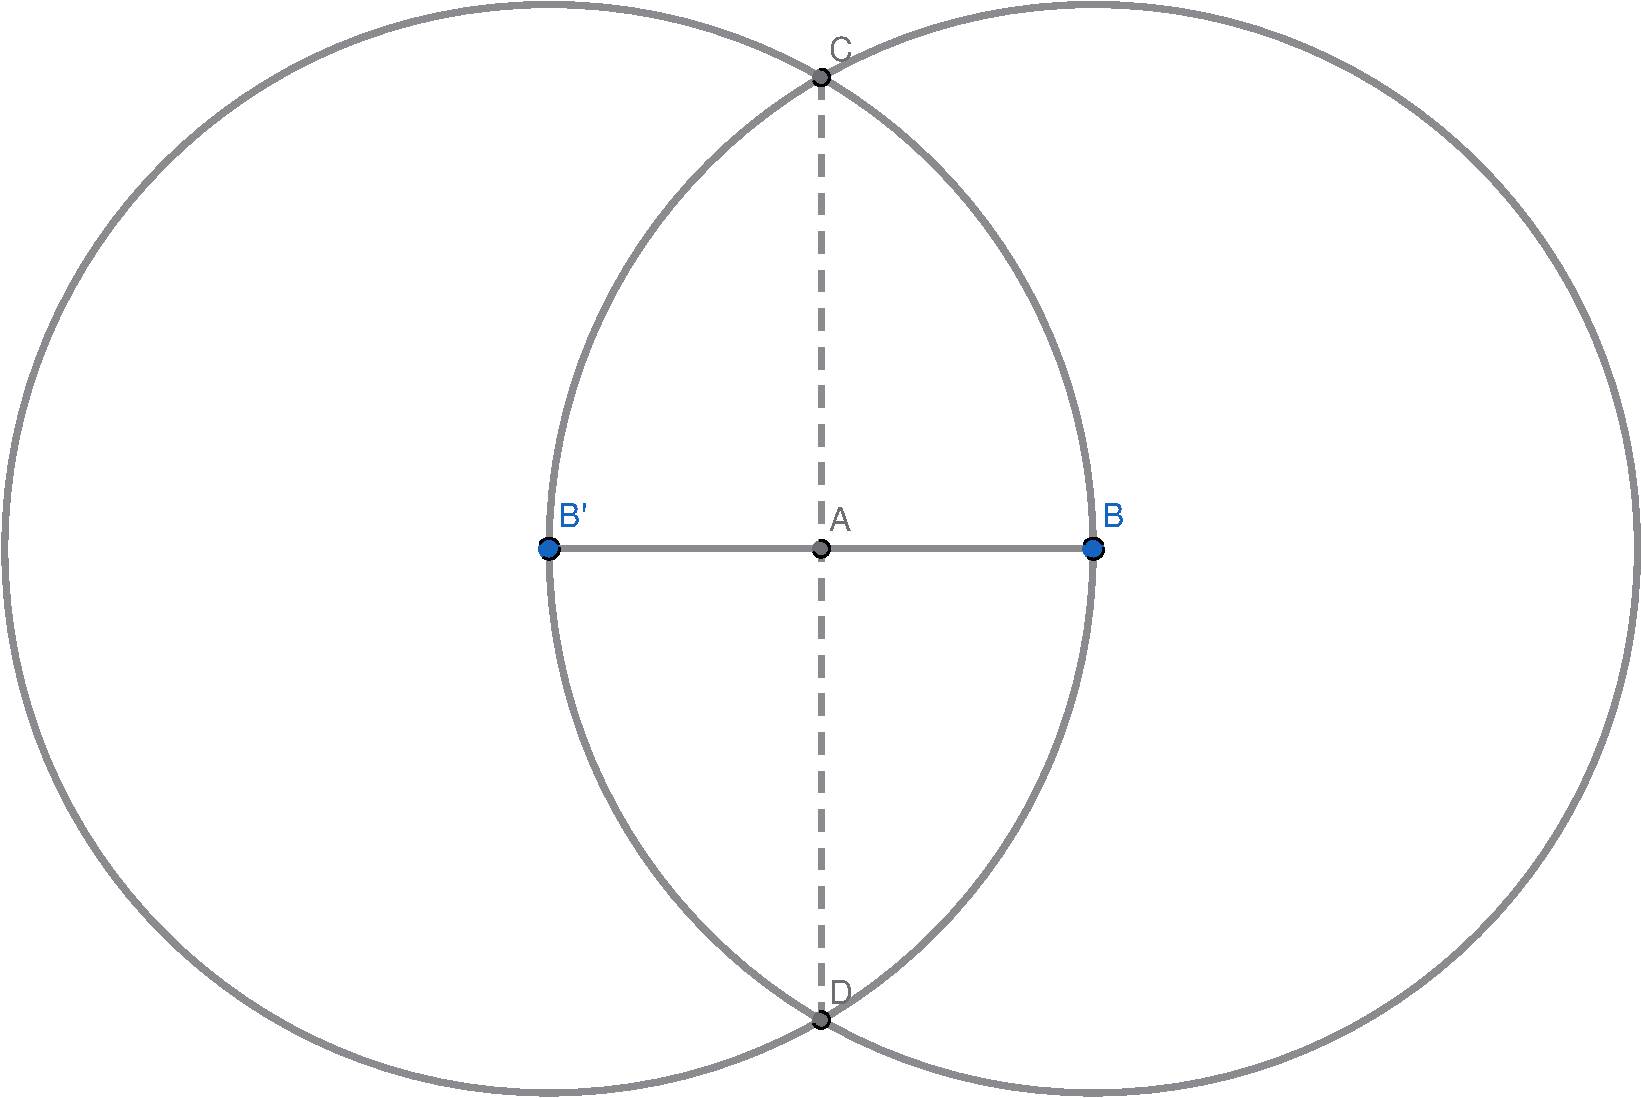
\includegraphics[scale=0.3]{img/perp}
 \captionof{figure}{作过定点的垂线}
 \label{fig:perp-of-point}
\end{center}
}
\end{Answer}

\ifx\wholebook\relax \else
\section{参考答案}
\shipoutAnswer

\subimport{inc/}{evenpfnum-zh-cn}

\begin{thebibliography}{99}
\subimport{inc/}{bib-zh-cn}
\end{thebibliography}

\expandafter\enddocument
\fi
